\documentclass[8pt]{beamer}
\usepackage[utf8]{inputenc}
\usepackage{xcolor}
\usepackage{colortbl}
\usepackage{epsfig}
% \usepackage{cancel}
\usepackage{ulem}
% \usepackage{threeparttable} % Joao Pela: 
\usepackage{amsmath}
\usepackage{hyperref}
\usepackage{appendixnumberbeamer}
% \usepackage{feynmp}         % For latex produced Feynman Diagrams

% Rule for feynmp diagrams to be considered graphics
% \DeclareGraphicsRule{*}{mps}{*}{}
% 
% % New compile sequence for feynmp
% \makeatletter
% \def\endfmffile{%
%   \fmfcmd{\p@rcent\space the end.^^J%
%           end.^^J%
%           endinput;}%
%   \if@fmfio
%     \immediate\closeout\@outfmf
%   \fi
%   \ifnum\pdfshellescape=\@ne
%     \immediate\write18{mpost \thefmffile}%
%   \fi}
% \makeatother

\usetheme{Madrid}

\author[J. Pela]{João Pela}
\title[MC VBF QCD]{MC VBF+MET QCD Samples Studies}
\institute[ICL]{Imperial College London}
\date{2014-02-09}

% The log drawn in the upper right corner.
\logo{\includegraphics[height=0.115\paperheight]{img/Logo_CMSICL.png}}

\begin{document}
\setlength{\unitlength}{1mm}

% ###################################################
\begin{frame}
  \titlepage
\end{frame}

% ###################################################
\begin{frame}{Today's presentation}
 
\begin{block}{Topics}
 
\begin{itemize}
  \item QCD VBF samples details
  \item Kinematics distributions
  \item Yields Comparison QCD Inclusive and VBF-like
  \item GenMET vs RecoMET Study
\end{itemize}
 
\end{block}

\end{frame}

% ###################################################
\begin{frame}{Introduction}


QCD are by far the most frequent processes in collisions at CMS. The elevated cross sections of such processes mean it is normally impossible to generate samples big enough to simulate 
significant amounts of of equivalent luminosity so they can be used in data analysis.

\begin{block}{Methodology}

In order to overcome this problem we generated MC QCD samples with MET plus VBF-like jets.
\begin{itemize}
  \item Real MET (vectorial sum of generator level neutrino $p_T$)
  \item VBF-like jets (AK5 generator level jets)
\end{itemize}

\end{block}

This type of event have a significantly smaller cross section and so to simulate high integrated luminosity samples. 
 
\end{frame}

% ###################################################
\begin{frame}{MC Filter Details}
 
\begin{block}{MC Filter: Vectorial sum of neutrino $E_T$}

  \begin{itemize}
     \item $\sum E_\perp(\vec{\nu}) > 40$ $GeV$
  \end{itemize}

\end{block}

\begin{block}{MC Filter: Dijet Filter}

  \begin{itemize}
    \item Select jets with:
    \begin{itemize}
      \item $p_\perp>20$ $GeV$
      \item $|\eta|<5.0$
    \end{itemize}
    \item From selected jets at least one pair with:
    \begin{itemize}
      \item $m_{jj}>700$ $GeV$
      \item $\Delta\eta>3.2$
    \end{itemize}    
  \end{itemize}

\end{block}

\end{frame}

% ###################################################
\begin{frame}{Sample Details}
 
Database URL: https://cmsdbsprod.cern.ch:8443/cms\_dbs\_ph\_analysis\_01\_writer/servlet/DBSServlet
 
\begin{block}

\resizebox{\linewidth}{!}{
\begin{tabular}{|c|l|}
\hline
Sample & Identifier \\
\hline \hline
QCD-Pt-80to120  & /VBFQCD\_Pt\_80to120\_MET40\_step1\_v1/pela-VBFQCD\_Pt\_80to120\_MET40\_step3\_v1-3664d28163503ca8171ba37083c39fc9/USER \\
QCD-Pt-120to170 & /VBFQCD\_Pt\_120to170\_MET40\_step1\_v1/pela-VBFQCD\_Pt\_120to170\_MET40\_step3\_v1-3664d28163503ca8171ba37083c39fc9/USER \\
QCD-Pt-170to300 & /VBFQCD\_Pt\_170to300\_MET40\_step1\_v1/pela-VBFQCD\_Pt\_170to300\_MET40\_step3\_v1-3664d28163503ca8171ba37083c39fc9/USER \\
QCD-Pt-300to470 & /VBFQCD\_Pt\_300to470\_MET40\_step1\_v1/pela-VBFQCD\_Pt\_470to600\_MET40\_step3\_v1-3664d28163503ca8171ba37083c39fc9/USER \\
QCD-Pt-470to600 & /VBFQCD\_Pt\_470to600\_MET40\_step1\_v1/pela-VBFQCD\_Pt\_470to600\_MET40\_step3\_v2-3664d28163503ca8171ba37083c39fc9/USER \\
\hline
\end{tabular}
}

\end{block}

\begin{block}
 
\begin{tabular}{|c|r|c|r|c|c|}
\hline
Sample          &       Ev. Gen. & Filter Eff. &  Events &  XS $[pb]$ & Eq. Lumi. $[fb^{-1}]$ \\
\hline \hline
QCD-Pt-80to120  & 39376000000 &    0.000049 & 1614416 &  1033680 &  38.09 \\
QCD-Pt-120to170 &  7000000000 &    0.000283 & 2051000 & 156293.3 &  44.79 \\
QCD-Pt-170to300 &  1375000000 &    0.000987 & 1391500 & 34138.15 &  40.28 \\
QCD-Pt-300to470 &    80000000 &    0.002659 &  207840 & 1759.549 &  45.47 \\
QCD-Pt-470to600 &    25000000 &    0.004127 &  104675 & 113.8791 & 219.53 \\
\hline
\end{tabular}

\end{block}

\end{frame}

% ###################################################
\begin{frame}{Kinematics Distributions}

\begin{columns}
\column[t]{0.25\linewidth}  
\begin{block}{$\Delta\eta$ cut: $Jet_1$ $p_T$}
 
\centering
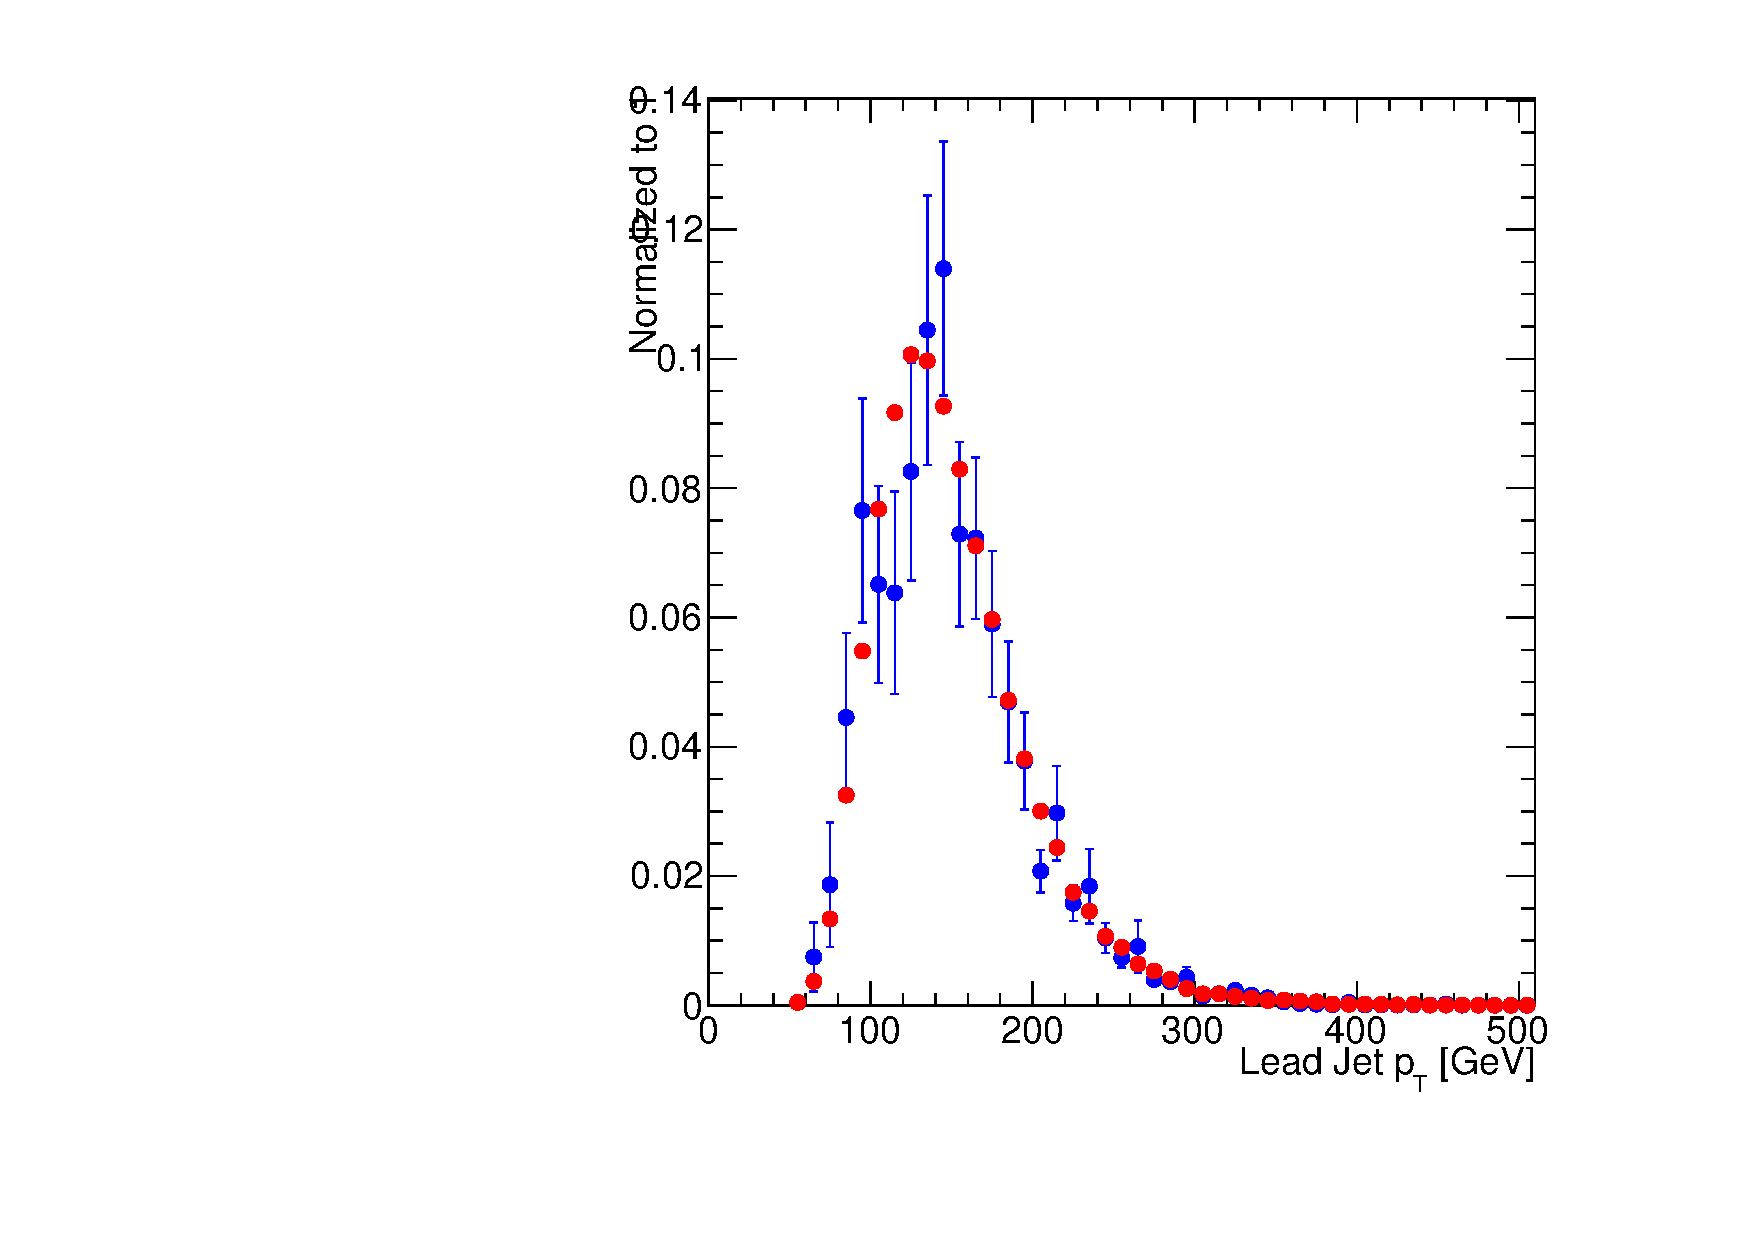
\includegraphics[width=\linewidth]{img/DEta_jpt_1.pdf} 
 
\end{block}

\begin{block}{$\Delta\eta$ cut: $Jet_1$ $\eta$}

\centering
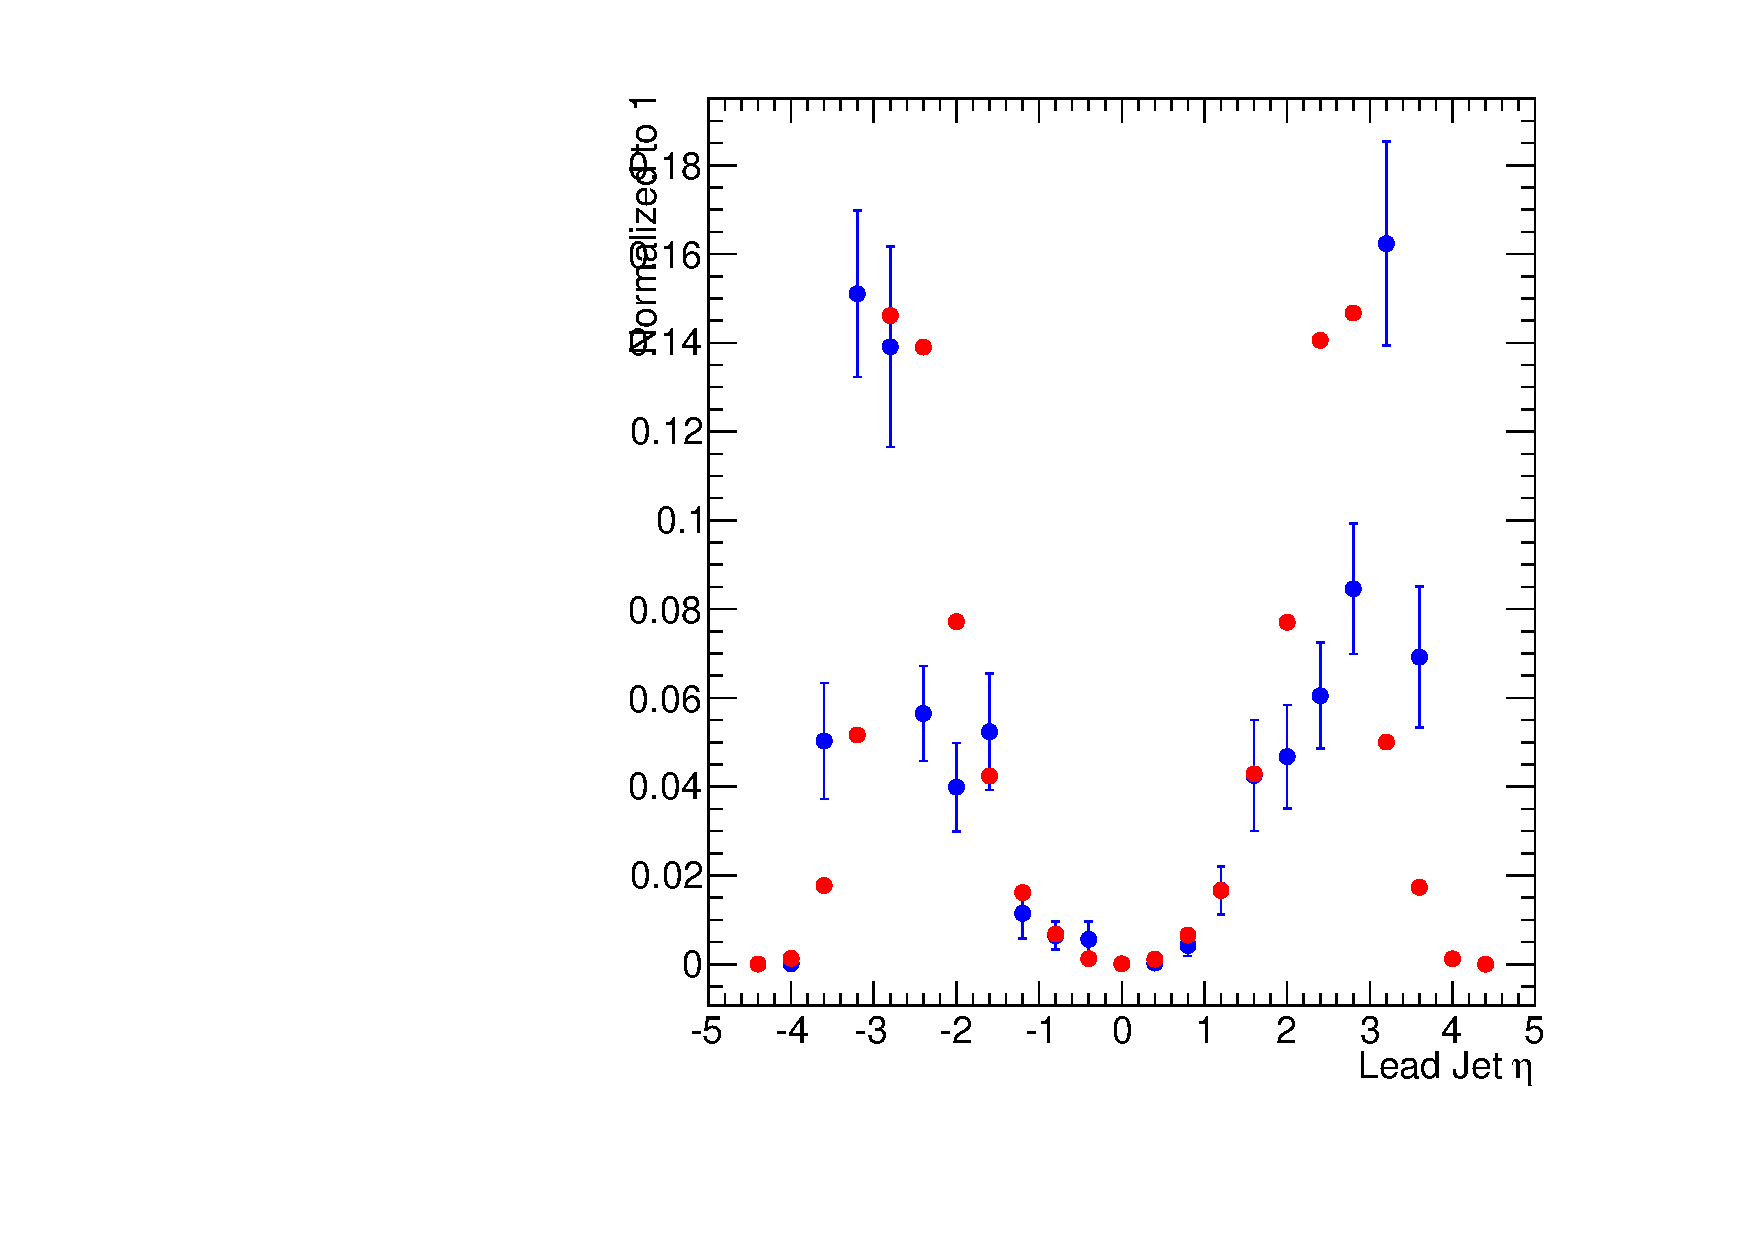
\includegraphics[width=\linewidth]{img/DEta_jeta_1.pdf} 
 
\end{block}

\column[t]{0.25\linewidth}  
\begin{block}{$\Delta\eta$ cut: $Jet_2$ $p_T$}

\centering 
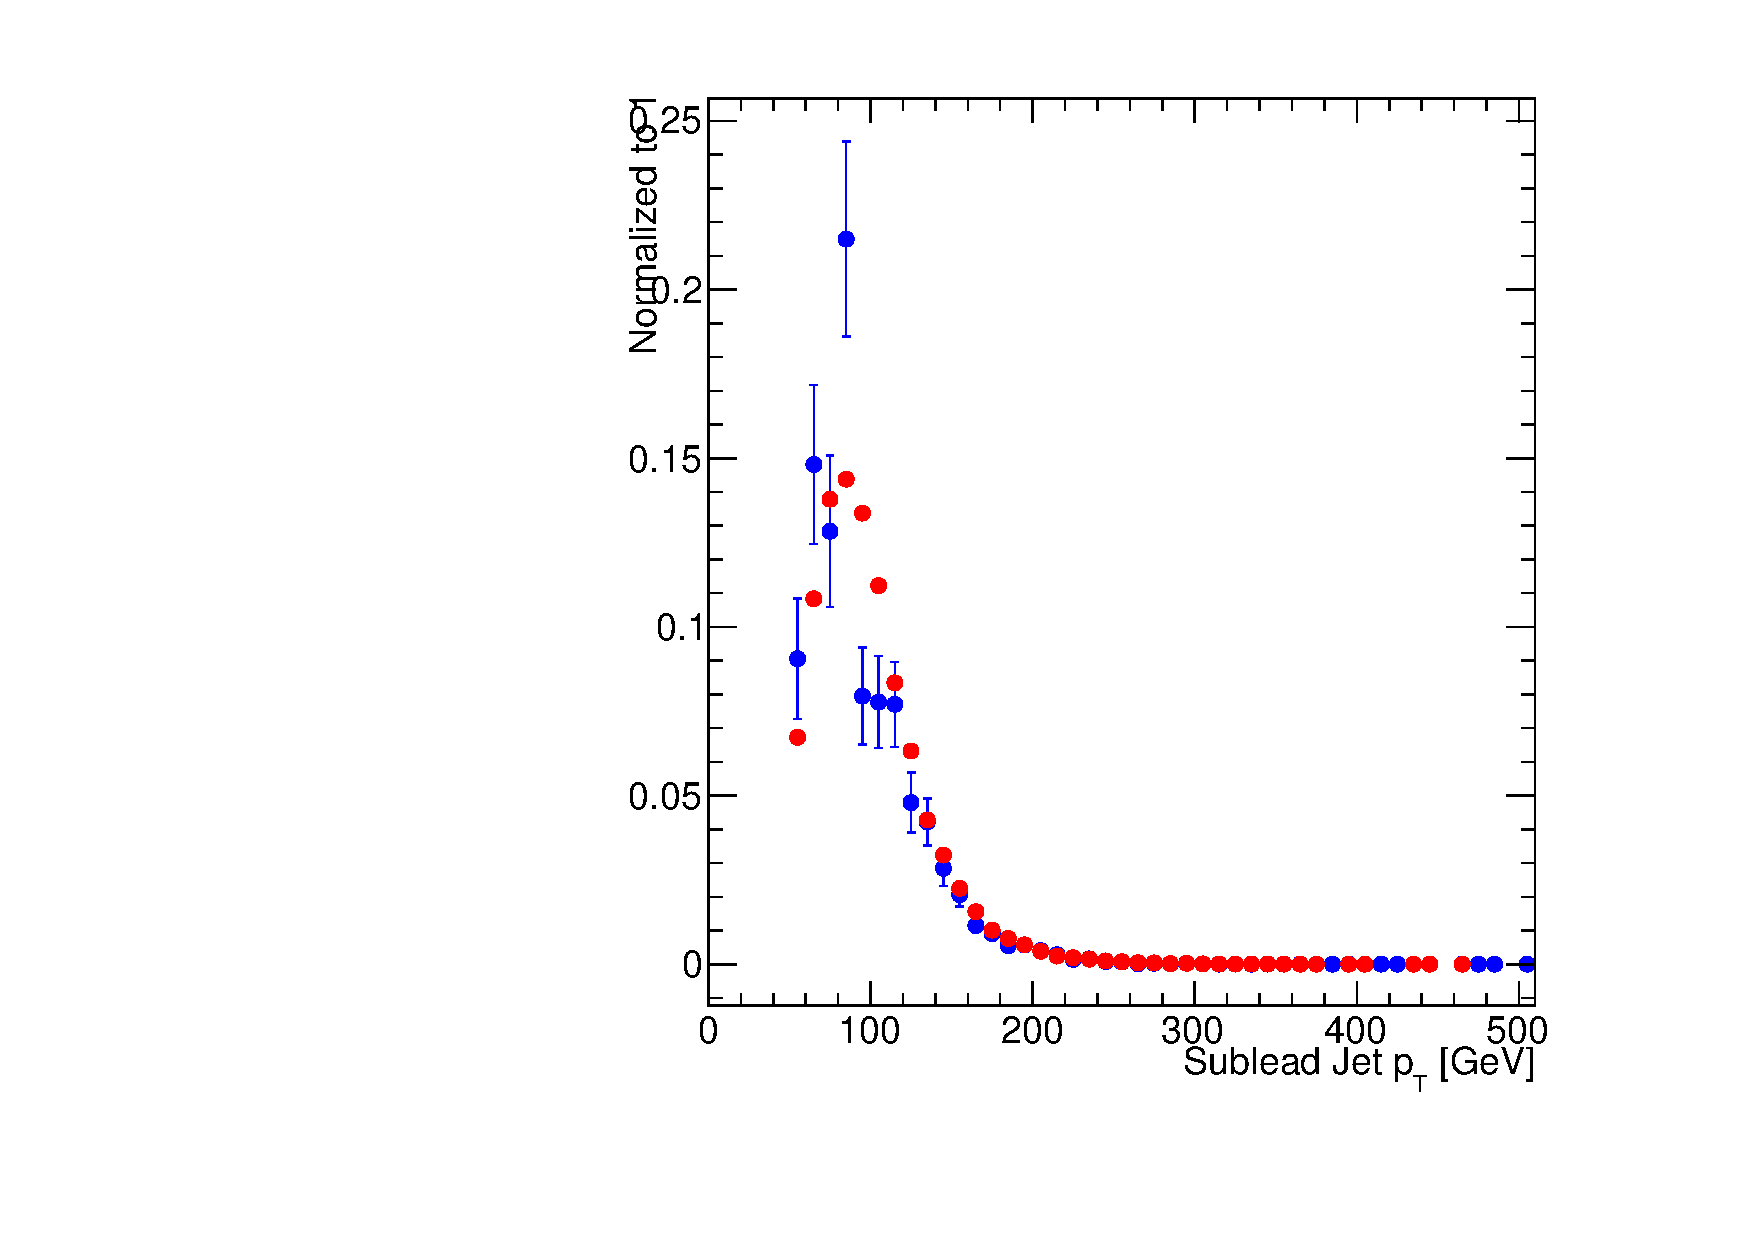
\includegraphics[width=\linewidth]{img/DEta_jpt_2.pdf} 
 
\end{block}

\begin{block}{$\Delta\eta$ cut: $Jet_2$ $\eta$}

\centering
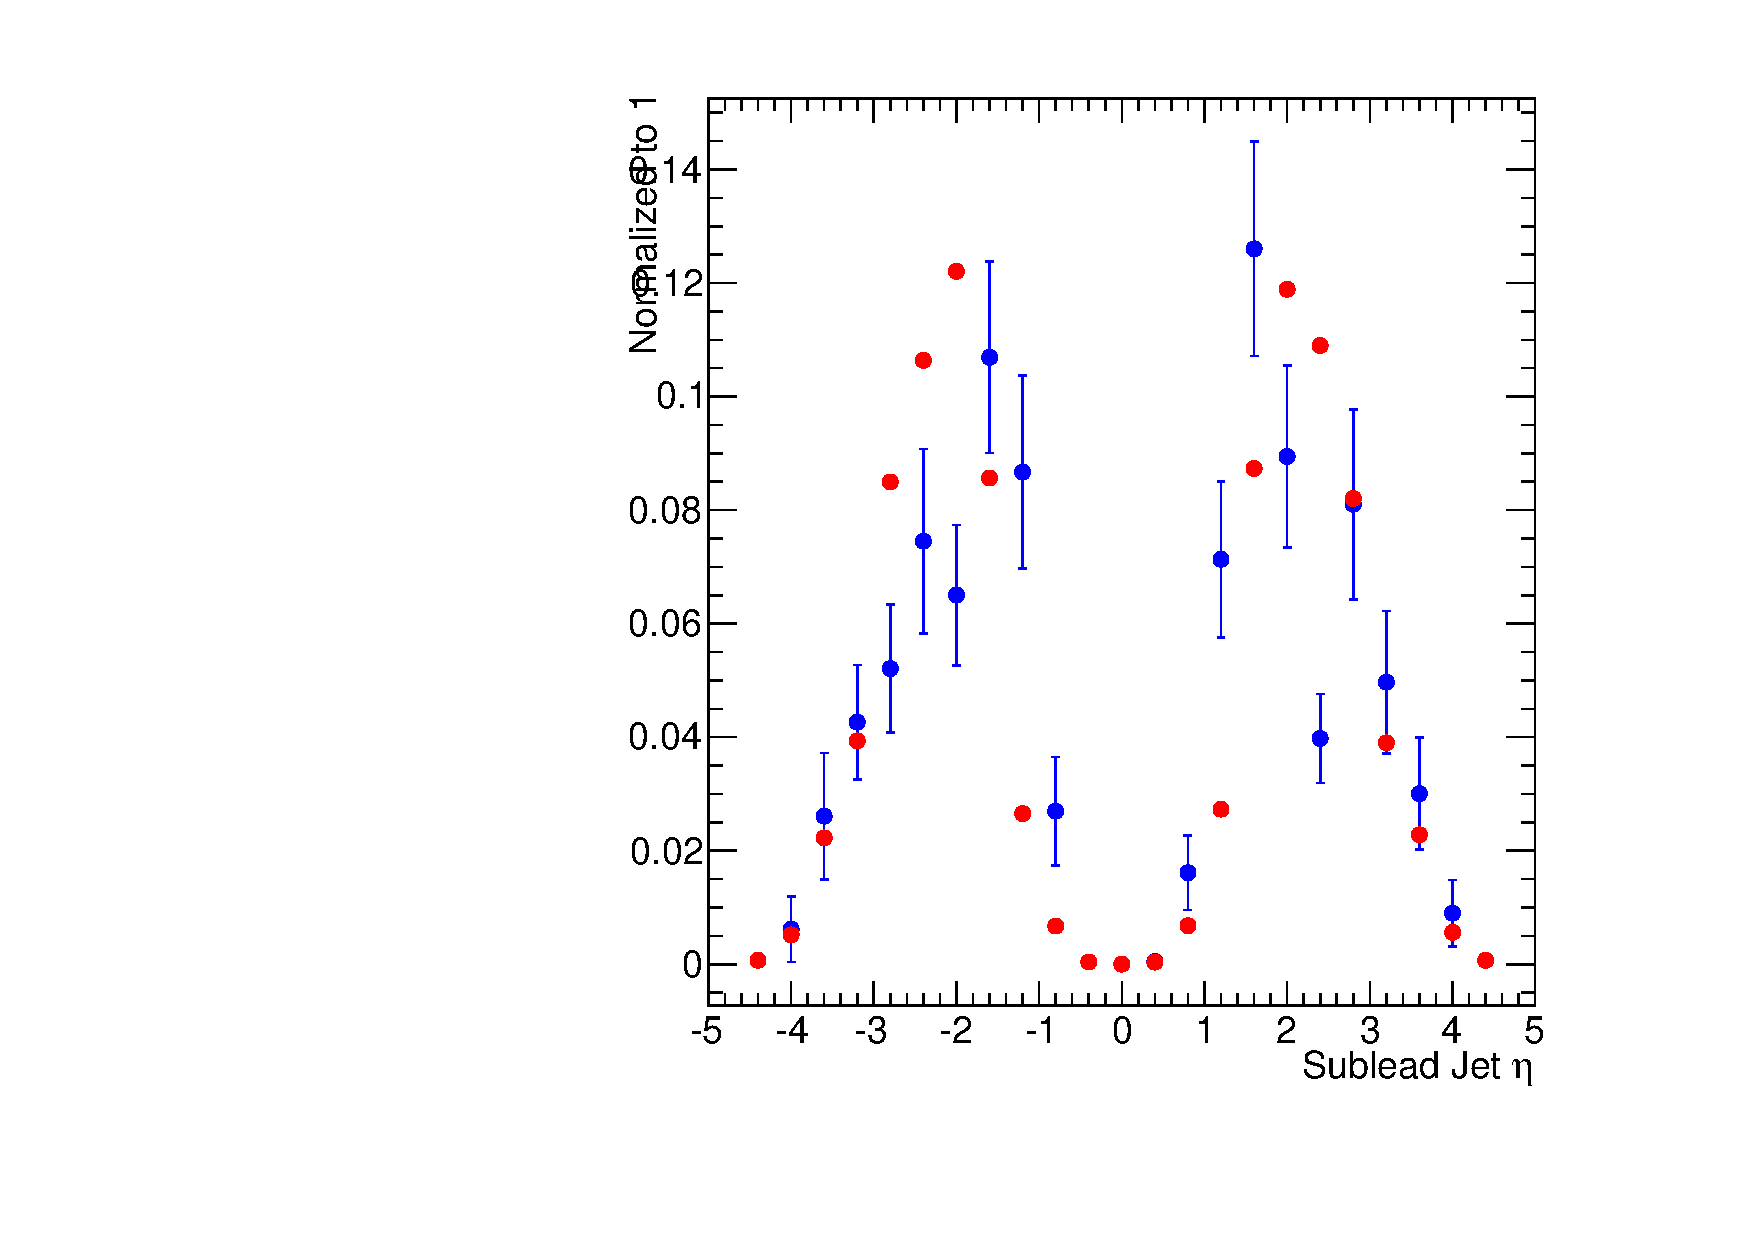
\includegraphics[width=\linewidth]{img/DEta_jeta_2.pdf} 
 
\end{block}

\column[t]{0.40\linewidth}  
\begin{block}
 
\begin{itemize}
  \item This plots are produced after jets selection ($p_{T}$ and $\eta$) and $\Delta\eta$ cuts over leading jets which is the last cut where we have
        significant statistics to compare Inclusive and VBF-like samples
  \item Legend:
  \begin{itemize}
    \item BLUE: QCD Inclusive
    \item RED: QCD VBF-like
  \end{itemize}
  \item Jet $p_T$, Jet $\eta$ variables seem o match to a reasonable level.
\end{itemize}

\end{block}

\end{columns}

\end{frame}



% ###################################################
\begin{frame}{Kinematics Distributions}

\begin{columns}
\column[t]{0.25\linewidth}  
\begin{block}{$\Delta\eta$ cut: MET}
 
\centering
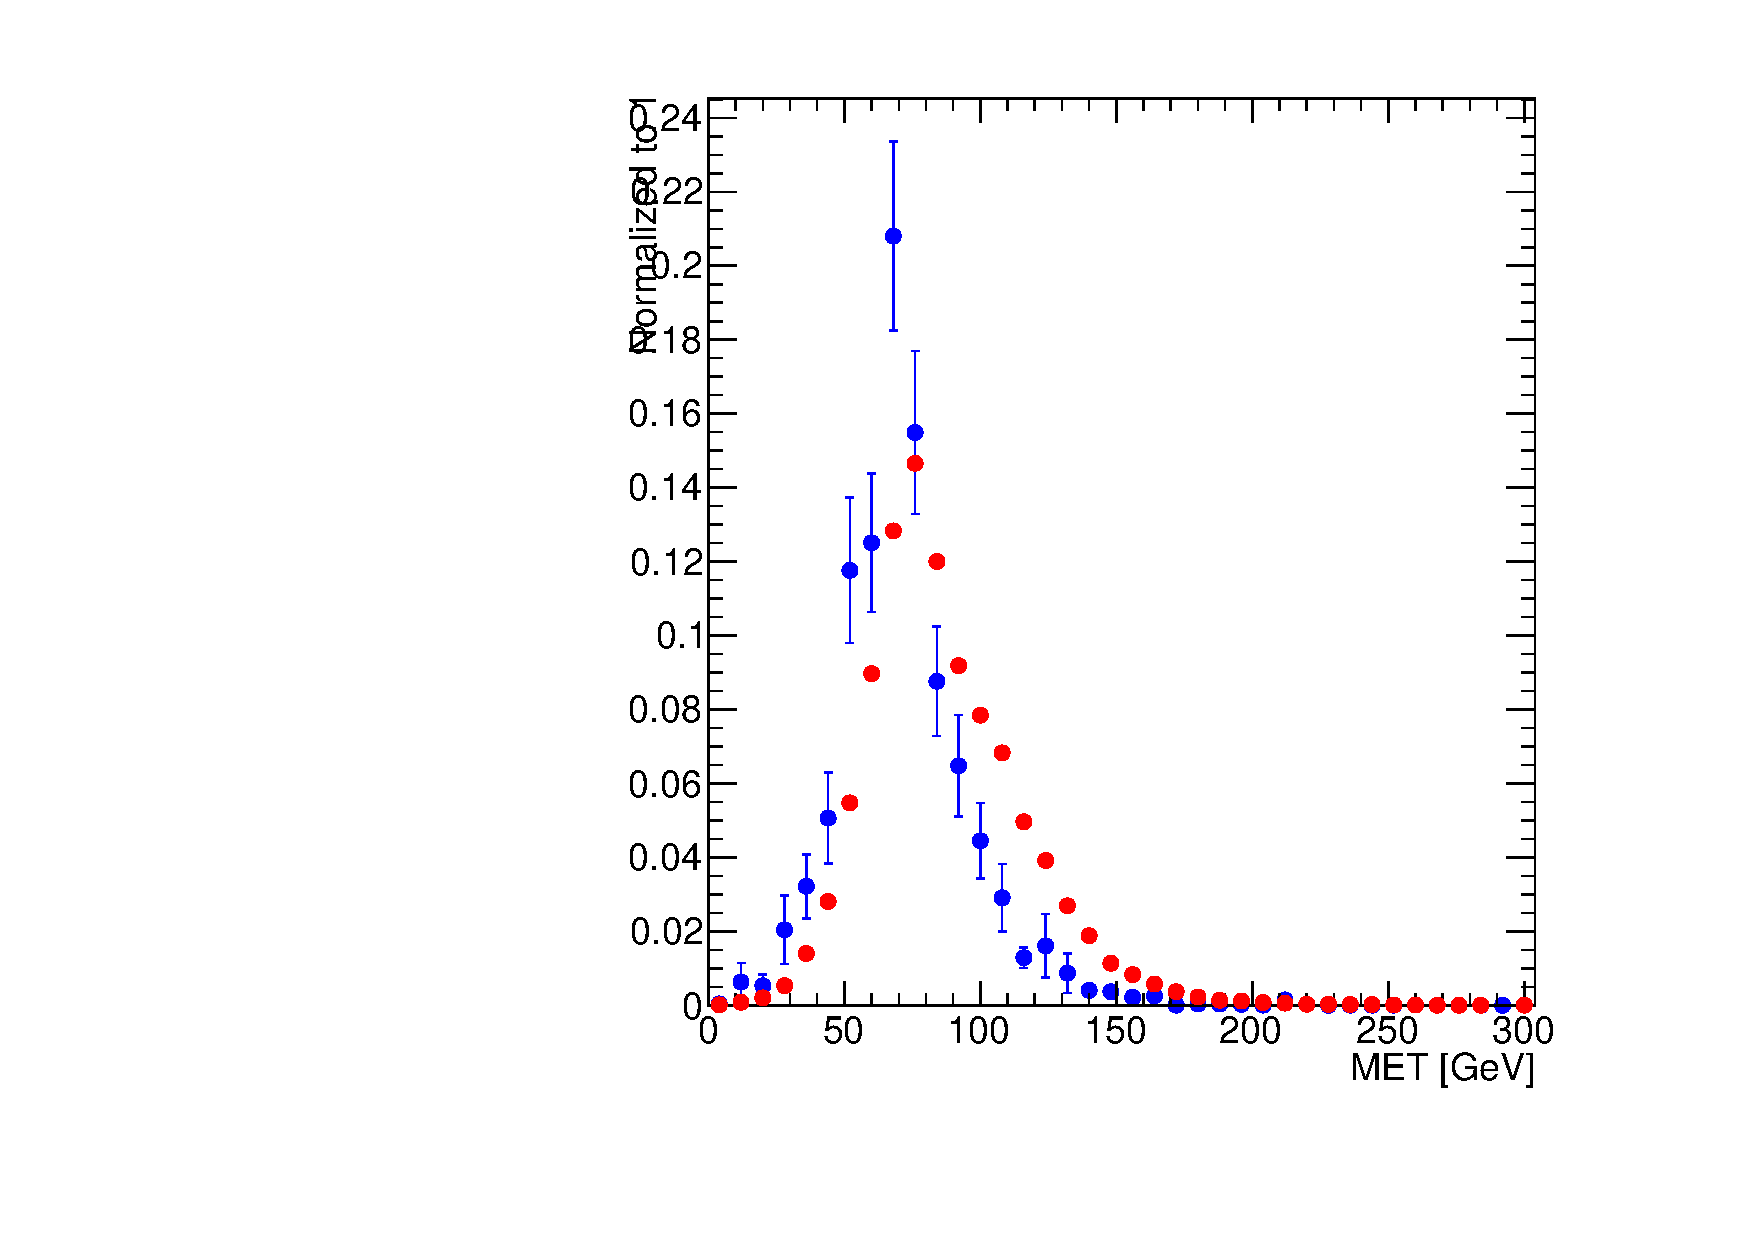
\includegraphics[width=\linewidth]{img/DEta_met.pdf} 
 
\end{block}

\begin{block}{$\Delta\eta$ cut: $M_{jj}$}

\centering
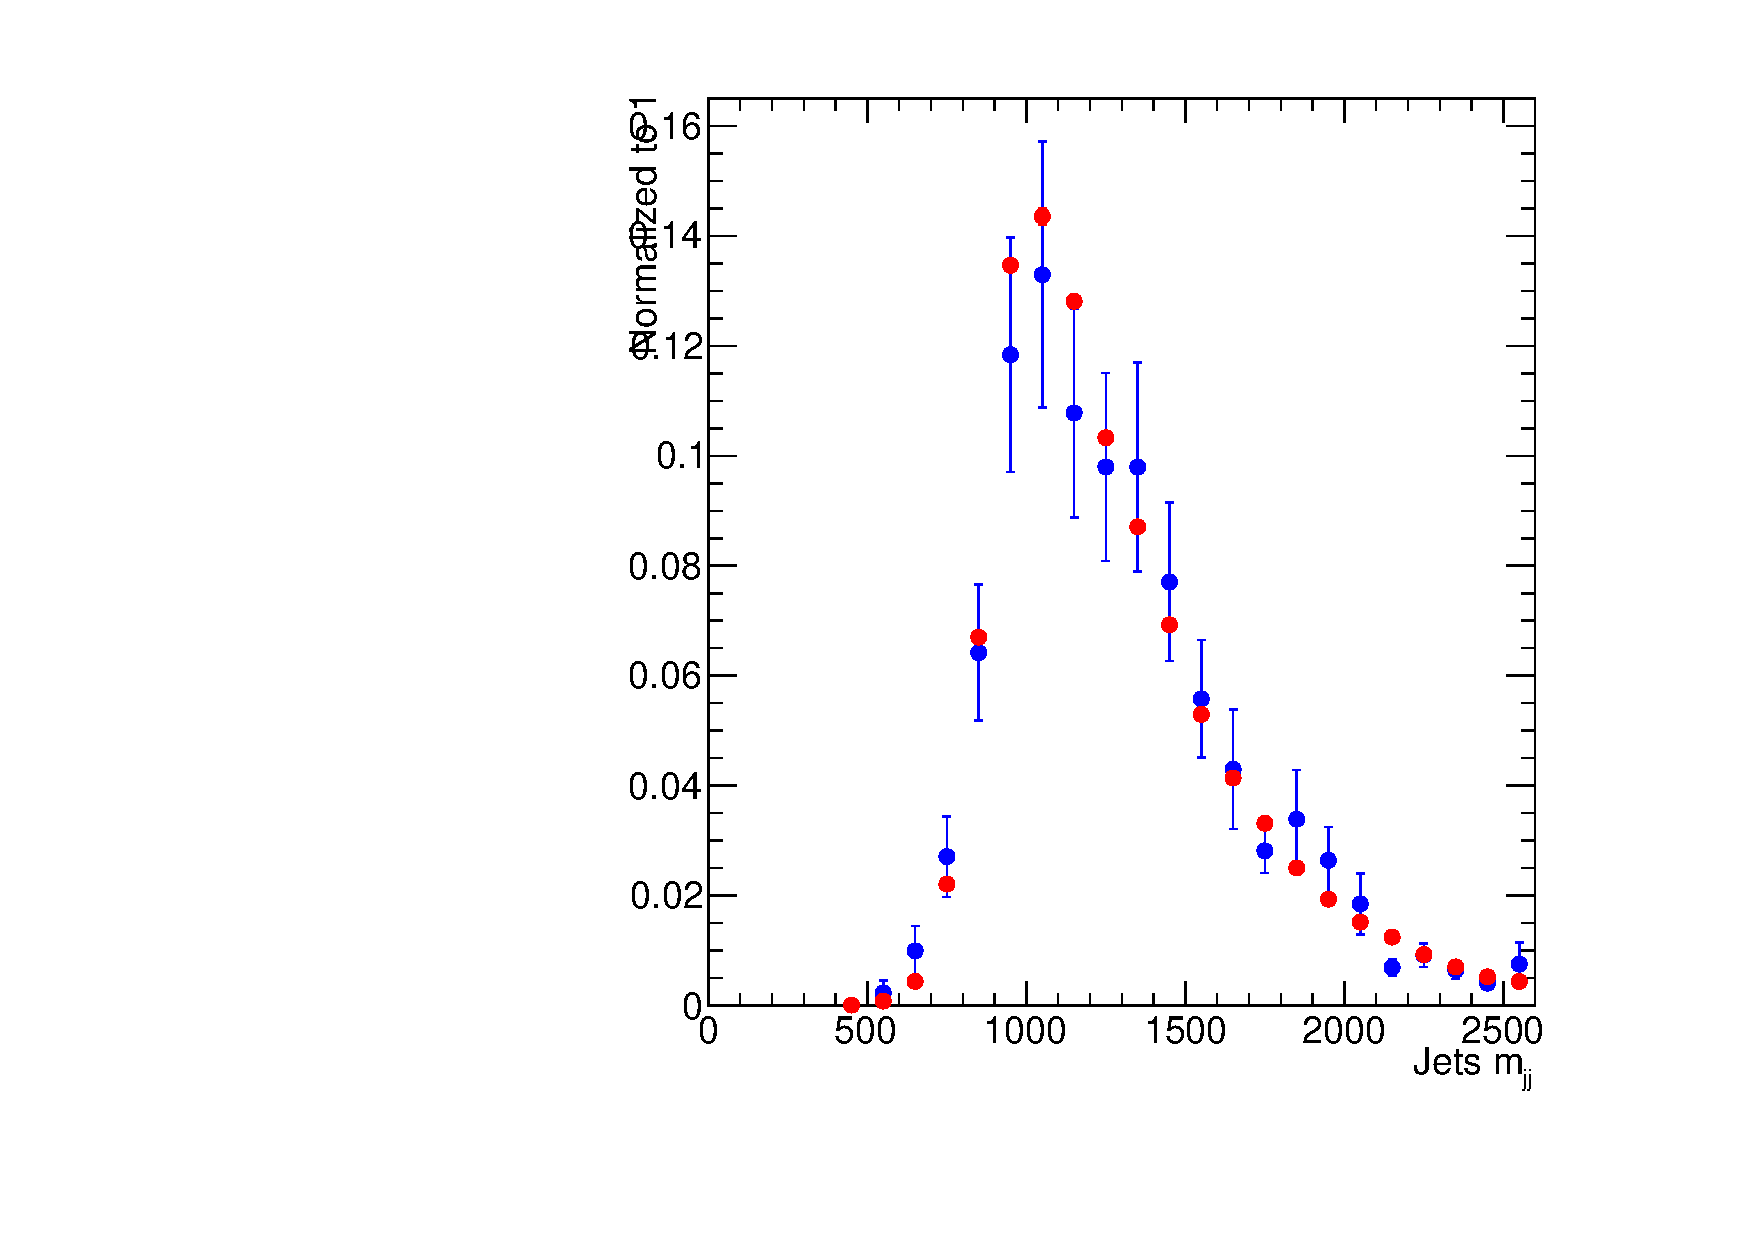
\includegraphics[width=\linewidth]{img/DEta_mjj.pdf} 
 
\end{block}


\column[t]{0.25\linewidth}  
\begin{block}{$\Delta\eta$ cut: $\Delta\Phi_{jj}$}
 
\centering
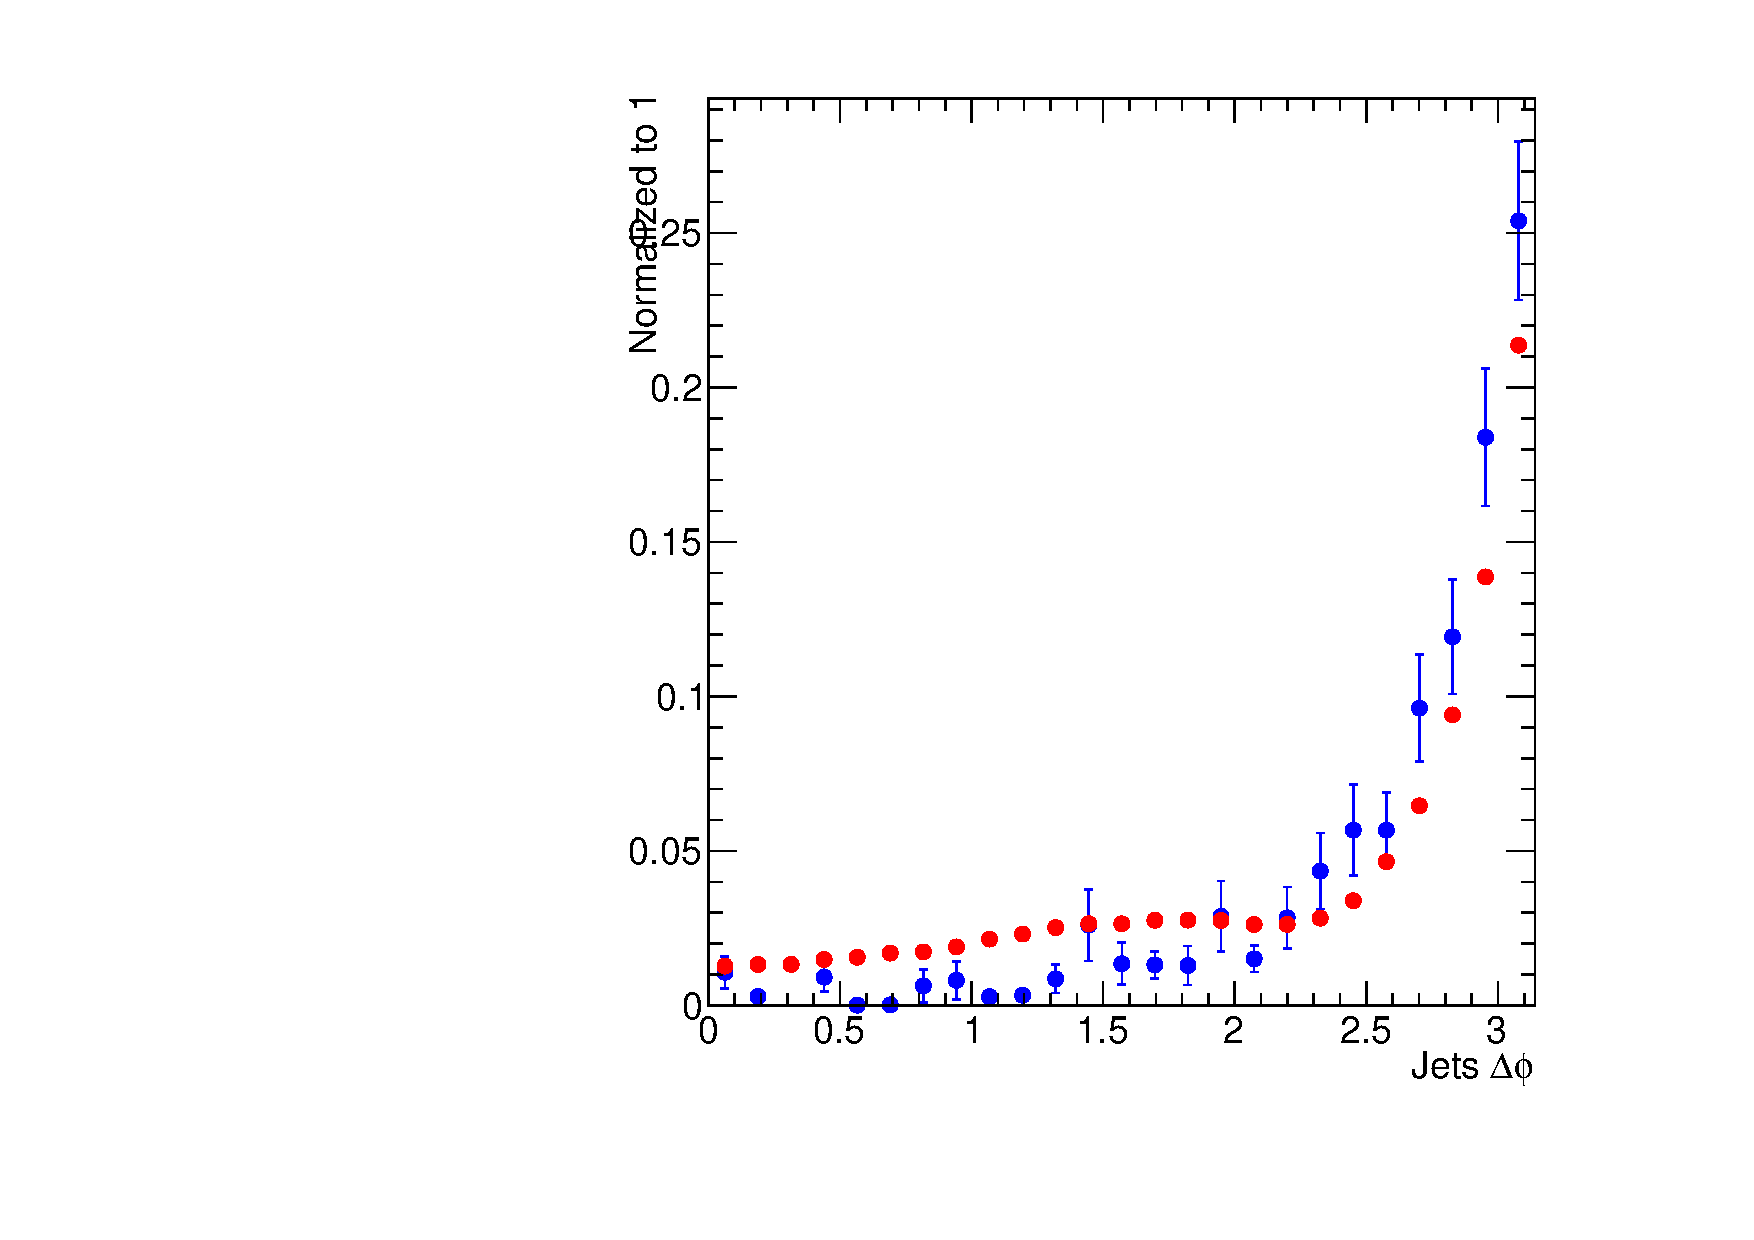
\includegraphics[width=\linewidth]{img/DEta_dphijj.pdf} 
 
\end{block}


\column[t]{0.40\linewidth}  
\begin{block}
 
\begin{itemize}
  \item This plots are produced after jets selection ($p_{T}$ and $\eta$) and $\Delta\eta$ cuts over leading jets which is the last cut where we have
        significant statistics to compare Inclusive and VBF-like samples
  \item Legend:
  \begin{itemize}
    \item BLUE: QCD Inclusive
    \item RED: QCD VBF-like
  \end{itemize}
  \item $m_{jj}$ variables seem o match to a reasonable level
  \item MET does not match well since we have not applied at least the MET cut yet.
  \item $\Delta\phi_{jj}$ seems to start to match but we can only compare with more cuts applied and at this level we will not have statistics anymore.
\end{itemize}

\end{block}

\end{columns}

\end{frame}


% ###################################################
\begin{frame}{MC Yields Comparison}

\begin{block}{Absolute Yields}
 
\centering
\resizebox{\linewidth}{!}{
\begin{tabular}{|c||cc||cc||cc||cc||cc|}
\hline
 & 80-120 & 80-120 & 120-170 & 120-170 & 170-300 & 170-300 & 300-470 & 300-470 & 470-600 & 470-600 \\
\hline
Sample & Inc & VBF & Inc & VBF & Inc & VBF & Inc & VBF & Inc & VBF \\
\hline \hline
HLTMetClean & 1509 & 118990 & 4595 & 257091 & 11866 & 271997 & 39157 & 56799 & 50413 & 28823 \\
JetPair & 587 & 71790 & 2337 & 163602 & 6405 & 168792 & 21505 & 32431 & 27991 & 16280 \\
DEta & 189 & 31982 & 543 & 43187 & 647 & 16988 & 354 & 539 & 35 & 38 \\
MET & 1 & 852 & 11 & 1948 & 39 & 1543 & 48 & 108 & 8 & 11 \\
TightMjj & 0 & 372 & 7 & 1231 & 35 & 1380 & 48 & 108 & 8 & 11 \\
CJVpass & 0 & 39 & 4 & 171 & 19 & 282 & 18 & 21 & 2 & 2 \\
DPhi & 0 & 12 & 0 & 18 & 0 & 6 & 0 & 0 & 0 & 0 \\
\hline
\end{tabular}

}
Number of entries for each QCD $p_T$ hat for after several cuts in current cut flow

\end{block}

\begin{block}{Weighted Yields}

\centering
\resizebox{\linewidth}{!}{
\begin{tabular}{|c||cc||cc||cc||cc||cc|}
\hline
 & 80-120 & 80-120 & 120-170 & 120-170 & 170-300 & 170-300 & 300-470 & 300-470 & 470-600 & 470-600 \\
\hline
Sample & Inc & VBF & Inc & VBF & Inc & VBF & Inc & VBF & Inc & VBF \\
\hline \hline
HLTMetClean & 2436603.32 & 55846.48 & 1446548.90 & 104815.88 & 957742.98 & 124768.50 & 166055.20 & 23030.77 & 21139.22 & 2394.68 \\
JetPair & 469225.26 & 12722.61 & 364877.70 & 27234.70 & 260740.43 & 35168.11 & 50960.28 & 6958.12 & 7709.01 & 934.73 \\
DEta & 276326.77 & 7371.62 & 142118.25 & 9995.54 & 42229.51 & 4987.06 & 1233.85 & 153.28 & 12.45 & 2.26 \\
MET & 1.50 & 300.35 & 4672.18 & 682.16 & 3577.84 & 661.70 & 232.67 & 43.28 & 4.06 & 0.82 \\
TightMjj & 0.00 & 154.99 & 3625.30 & 464.06 & 3309.76 & 597.43 & 232.67 & 43.28 & 4.06 & 0.82 \\
CJVpass & 0.00 & 15.17 & 1858.14 & 63.84 & 1773.69 & 118.74 & 81.75 & 9.61 & 0.92 & 0.19 \\
DPhi & 0.00 & 5.10 & 0.00 & 8.23 & 0.00 & 2.53 & 0.00 & 0.00 & 0.00 & 0.00 \\
\hline
\end{tabular}

}
Weighted (trigger, PU, ID, cross section) number of events for each QCD $p_T$ hat for after several cuts in current cut flow.

\end{block}

\end{frame}

% ###################################################
\begin{frame}{Some Conclusions}

\begin{block}{Conclusions}
 
\begin{itemize}
  \item Kinematics shapes seem to tend to match to inclusive samples after a few cuts are applied.
  \item After all selection cuts have been applied (even after MET cut) it is difficult to compare samples because QCD Inclusive sample become heavily suppressed.
  \item How ever there are significant yield differences specially evident in the QCD 470-600 $GeV$ where QCD Inc samples have statistics comparable with 2012 data.
\end{itemize}

\end{block}

\begin{block}{Plans}
 
\begin{itemize}
  \item It was suggested that this discrepancies may be cause by fake MET events. So I started a GenMET vs RecoMET study.
  \item Because QCD Inclusive samples are not enough, we need to compare QCD VBF-like samples with data, for this we need to choose a QCD dominated region.
\end{itemize}

\end{block}

\end{frame}

% ###################################################
\begin{frame}{Fake met contribution study}
 
To evaluate how much events pass out analysis cut of $MET>130$ $GeV$ that have a significant contribution of fake MET 
which the new QCD VBF-like samples will not be able to simulate we need to look at the inclusive samples.

\begin{columns}
 
\column[t]{0.45\linewidth}  
\begin{block}{Area Definition}
 
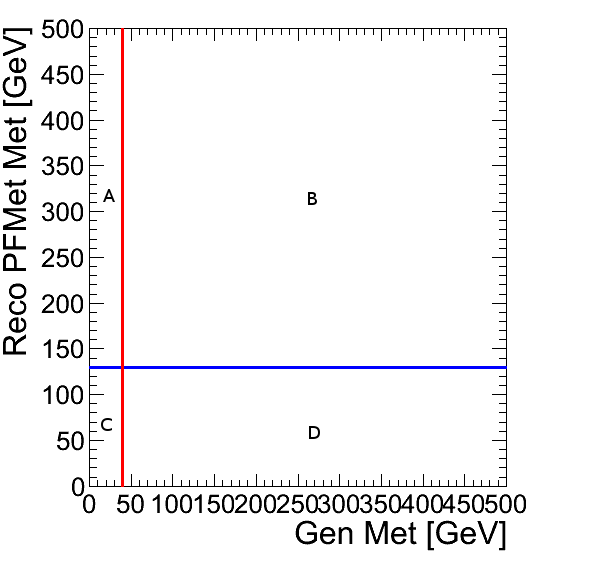
\includegraphics[width=\linewidth]{img/basic.png}
 
\end{block}

\column[t]{0.45\linewidth}  
\begin{block}
 
We can define 4 areas:
\begin{itemize}
 \item A: Accepted by Analysis MET cut but rejected by GenMET Filter
 \item B: Accepted by Analysis MET cut and accepted by GenMET Filter
 \item C: Rejected by Analysis MET cut and rejected by GenMET Filter
 \item D: Rejected by Analysis MET cut but accepted by GenMET Filter
\end{itemize}

From this we can define the B area normalization factor as $\frac{A+B}{B}$

\end{block}

\end{columns}

\end{frame}

% ###################################################
\begin{frame}{Gen Met Vs Reco MET I}

Plots here do now have any weighting but cross section since filters will operate over genEvents with no weigting this (so this is just a scaling).
Plot on the right Adds all the QCD inclusive $p_T$ hats taking into account the relative cross section.

\begin{columns}

\column[t]{0.45\linewidth}  
\begin{block}{QCD Inc 80-600 $GeV$}
 
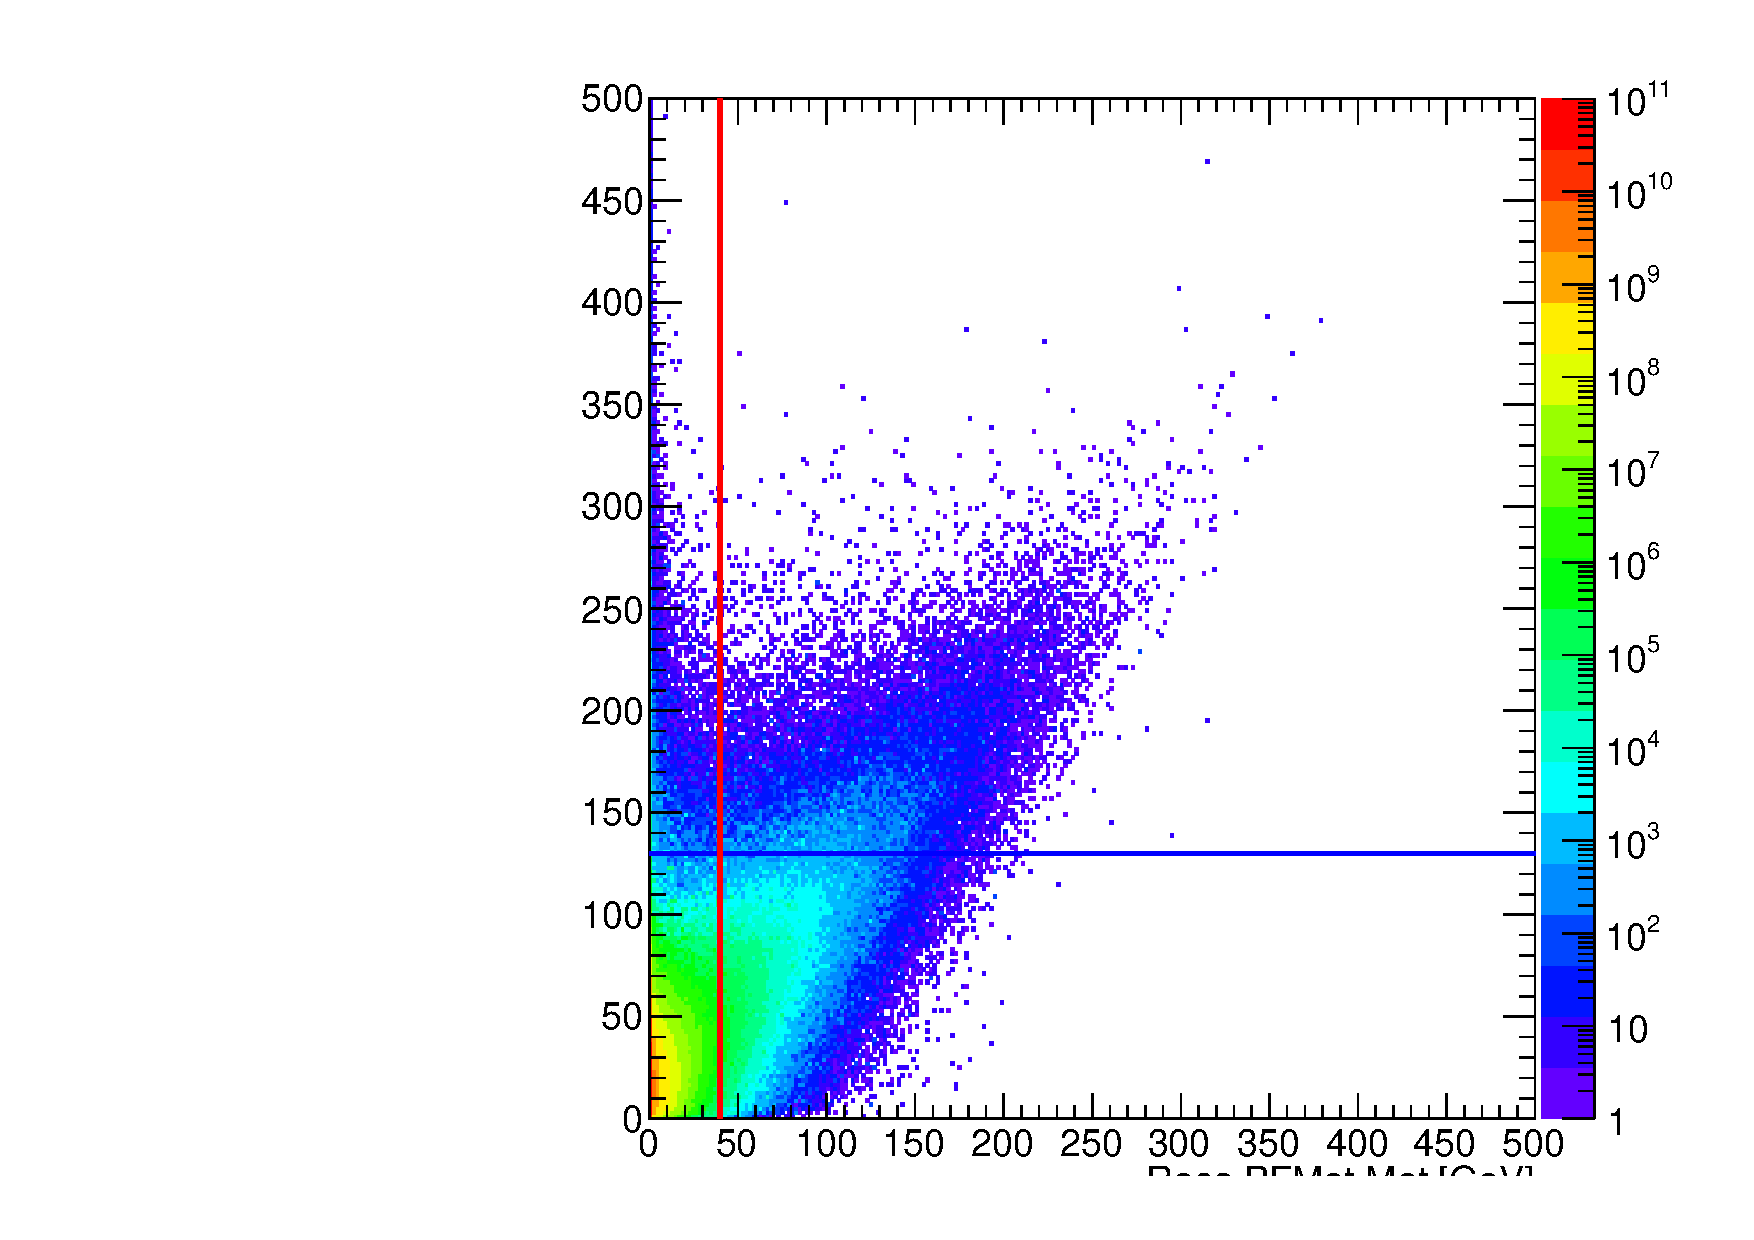
\includegraphics[width=\linewidth]{img/MC_QCDIncAll_GenVsReco_met}
 
\end{block}

\column[t]{0.45\linewidth} 
\begin{block}

\begin{itemize}
  \item There are clearly 2 population
  \begin{itemize}
    \item Events with real met along the diagonal of the plot
    \item Events with fake met along 0 gen MET vertical line
  \end{itemize}
  \item VBF samples only have events present on B area
\end{itemize}
 
\end{block}

\end{columns}

We can see in both plots that there is a significant population in both areas A and B.

\end{frame}

% ###################################################
\begin{frame}{Gen Met Vs Reco MET - Into Numbers}

Now we can calculate what is the percentage of events in each area and the normalization factor for B are.

\begin{block}{Areas and normalization factor}

\begin{table}[!h]
\centering
\resizebox{\linewidth}{!}{
\begin{tabular}{|c||c|c|c|c||c|}
\hline
Sample & A & B & C & D & Factor \\
\hline \hline
MC\_QCD-Pt-30to50-pythia6 & 0.000000 & 0.000000 & 0.999997 & 0.000003 & inf \\
MC\_QCD-Pt-50to80-pythia6 & 0.000000 & 0.000000 & 0.999884 & 0.000116 & nan \\
MC\_QCD-Pt-80to120-pythia6 & 0.000006 & 0.000001 & 0.998800 & 0.001193 & 5.625 \\
MC\_QCD-Pt-120to170-pythia6 & 0.000065 & 0.000024 & 0.995715 & 0.004195 & 3.676 \\
MC\_QCD-Pt-170to300-pythia6 & 0.000684 & 0.000281 & 0.989966 & 0.009069 & 3.432 \\
MC\_QCD-Pt-300to470-pythia6 & 0.005185 & 0.002331 & 0.976764 & 0.015721 & 3.224 \\
MC\_QCD-Pt-470to600-pythia6 & 0.016652 & 0.005900 & 0.959474 & 0.017973 & 3.823 \\
MC\_QCD-Pt-600to800-pythia6 & 0.034093 & 0.008591 & 0.939409 & 0.017906 & 4.969 \\
MC\_QCD-Pt-800to1000-pythia6 & 0.068863 & 0.011177 & 0.903115 & 0.016845 & 7.161 \\
MC\_QCD-Pt-1000to1400-pythia6 & 0.117719 & 0.012717 & 0.854500 & 0.015063 & 10.257 \\
MC\_QCD-Pt-1400to1800-pythia6 & 0.202556 & 0.014259 & 0.770444 & 0.012741 & 15.206 \\
MC\_QCD-Pt-1800-pythia6 & 0.285060 & 0.015070 & 0.688829 & 0.011041 & 19.916 \\
\hline \hline
Total & 0.000001 & 0.000000 & 0.999954 & 0.000044 & 4.761343 \\
\hline
\end{tabular}

}
\caption{Relative are for A, B, C and D areas and factor to normalize B area to A+B (normalize QCD VBF samples to inclusive at $MET>130$ $GeV$ cut.}
\end{table}

\end{block}

The normalization factors seem to be approximatly of the order of the discrepancy in yields seen last week.

\end{frame}

% ###################################################
\begin{frame}{Aplying Factors to last week tables}

Considerations
\begin{itemize}
  \item Factors are calculated for uncorrected (PU, Trigger and ID) events and applied to tables from last week which
        is to some level \uline{wrong} but at first approximation gives an idea of the effect of this normalization factors.
  \item Factors only acount for events lost due to fake MET which is just one of the 2 filters applied, the VBF QCD jets filters
        while have its own losses which need to be accounted in parallel.
\end{itemize}

\begin{block}{Correcting a MET cut level}

\resizebox{\linewidth}{!}{
\begin{tabular}{|c||cc||cc||cc||cc||cc|}
\hline
 & 80-120 & 80-120 & 120-170 & 120-170 & 170-300 & 170-300 & 300-470 & 300-470 & 470-600 & 470-600 \\
\hline
Cut                & Inc  &     VBF &     Inc &     VBF &     Inc &     VBF &    Inc &    VBF &  Inc & VBF \\
\hline \hline
MET (Last Week)    & 1.50 &  300.35 & 4672.18 &  682.16 & 3577.84 &  661.70 & 232.67 &  43.28 & 4.06 & 0.82 \\
MET (Apply factor) & 1.50 & 1689.46 & 4672.18 & 2507.62 & 3577.84 & 2270.95 & 232.67 & 139.53 & 4.06 & 3.13 \\
\hline
\end{tabular}
}

\end{block}

Number are now much closer to match, execept on the 80-120 $GeV$ bin where QCD inclusive only has one event highly suppressed but non xsec weights. 
Note bin 470-600 $GeV$ where both QCD Inc and QCD VBF have enough statistics to simulate 20 $fb^{-1}$ now are much closer.


\end{frame}

% ###################################################
\begin{frame}{Summary and next steps}
 
\begin{block}{Summary:}
 
\begin{itemize}
  \item QCD VBF samples show some promise in describing the QCD contribution to our analysis (some event on the sample pass the whole selection)
  \item There is some discrepancy on the comparison between QCD Inclusive and VBF-like samples but that seams to be due to fake met contribution.
  \item the GenMET vs RecoMET study clearly showed that we have 2 population of events real and fake met which are clearly separated which gives us hope that we may able to suppress the fake met events.
\end{itemize}

\end{block}

\begin{block}{Next Steps:}
 
\begin{itemize}
 \item Add genJets filter study in order to fully understand VBF-like sample
 \item Compare QCD VBF-like sample with data in QCD dominated regions
 \item Determine sample normalization from data
 \item Attempt to suppress fake met population (in QCD Inclusive sample) using MVA or variables (MET significance, MET-Dijet angle, etc) to suppress regions sample cannot model.
\end{itemize}
 
\end{block}

\end{frame}


% ###################################################
\appendix
% ###################################################
\begin{frame}
 
\begin{block}

\begin{center}Backup Slides\end{center}

\end{block}

\end{frame}

% ###################################################
\begin{frame}{Gen Met Vs Reco MET I}

Plots here do now have any weighting but cross section since filters will operate over genEvents with no weigting this (so this is just a scaling).

\begin{columns}
    
\column[t]{0.45\linewidth}  
\begin{block}{80to120}
 
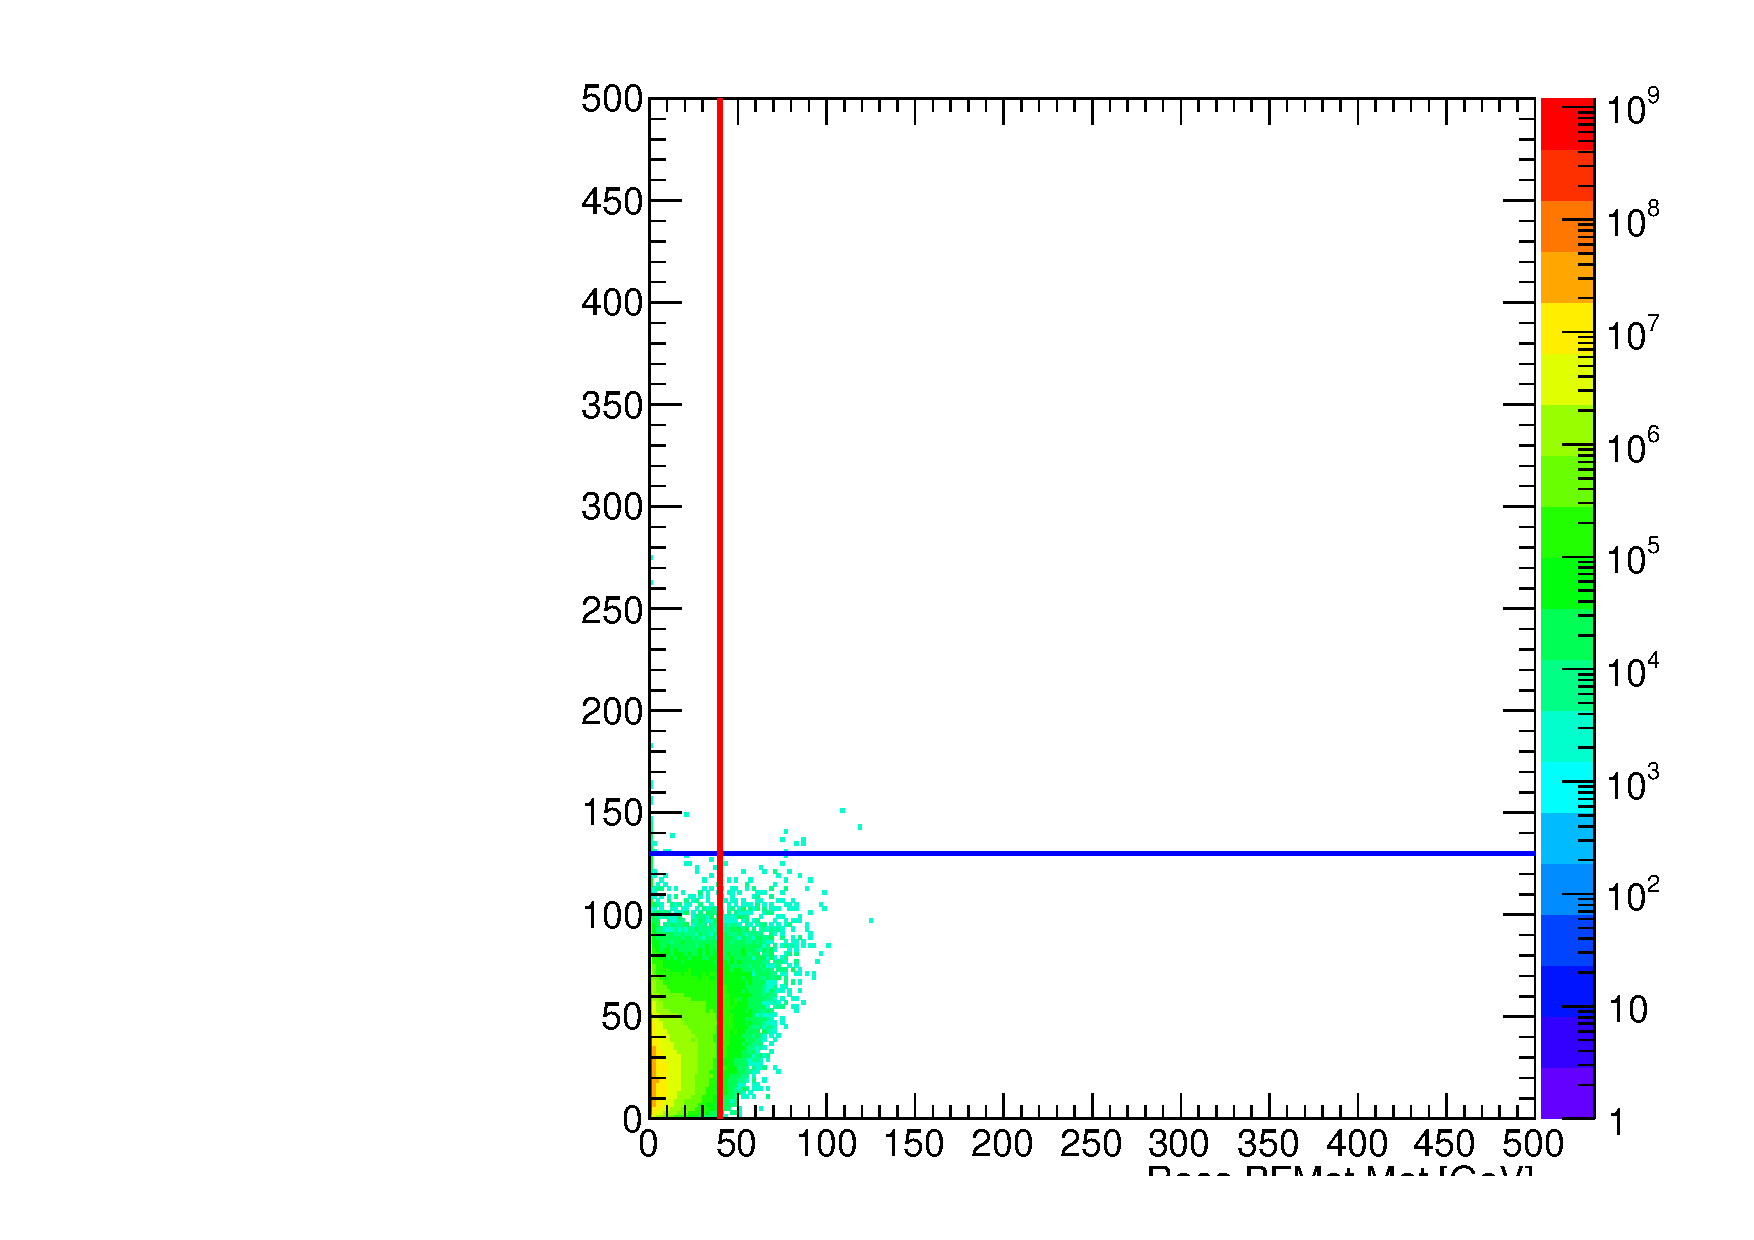
\includegraphics[width=\linewidth]{img/MC_QCD-Pt-80to120-pythia6_GenVsReco_met}

\end{block}

\column[t]{0.45\linewidth}  
\begin{block}{120to170}
 
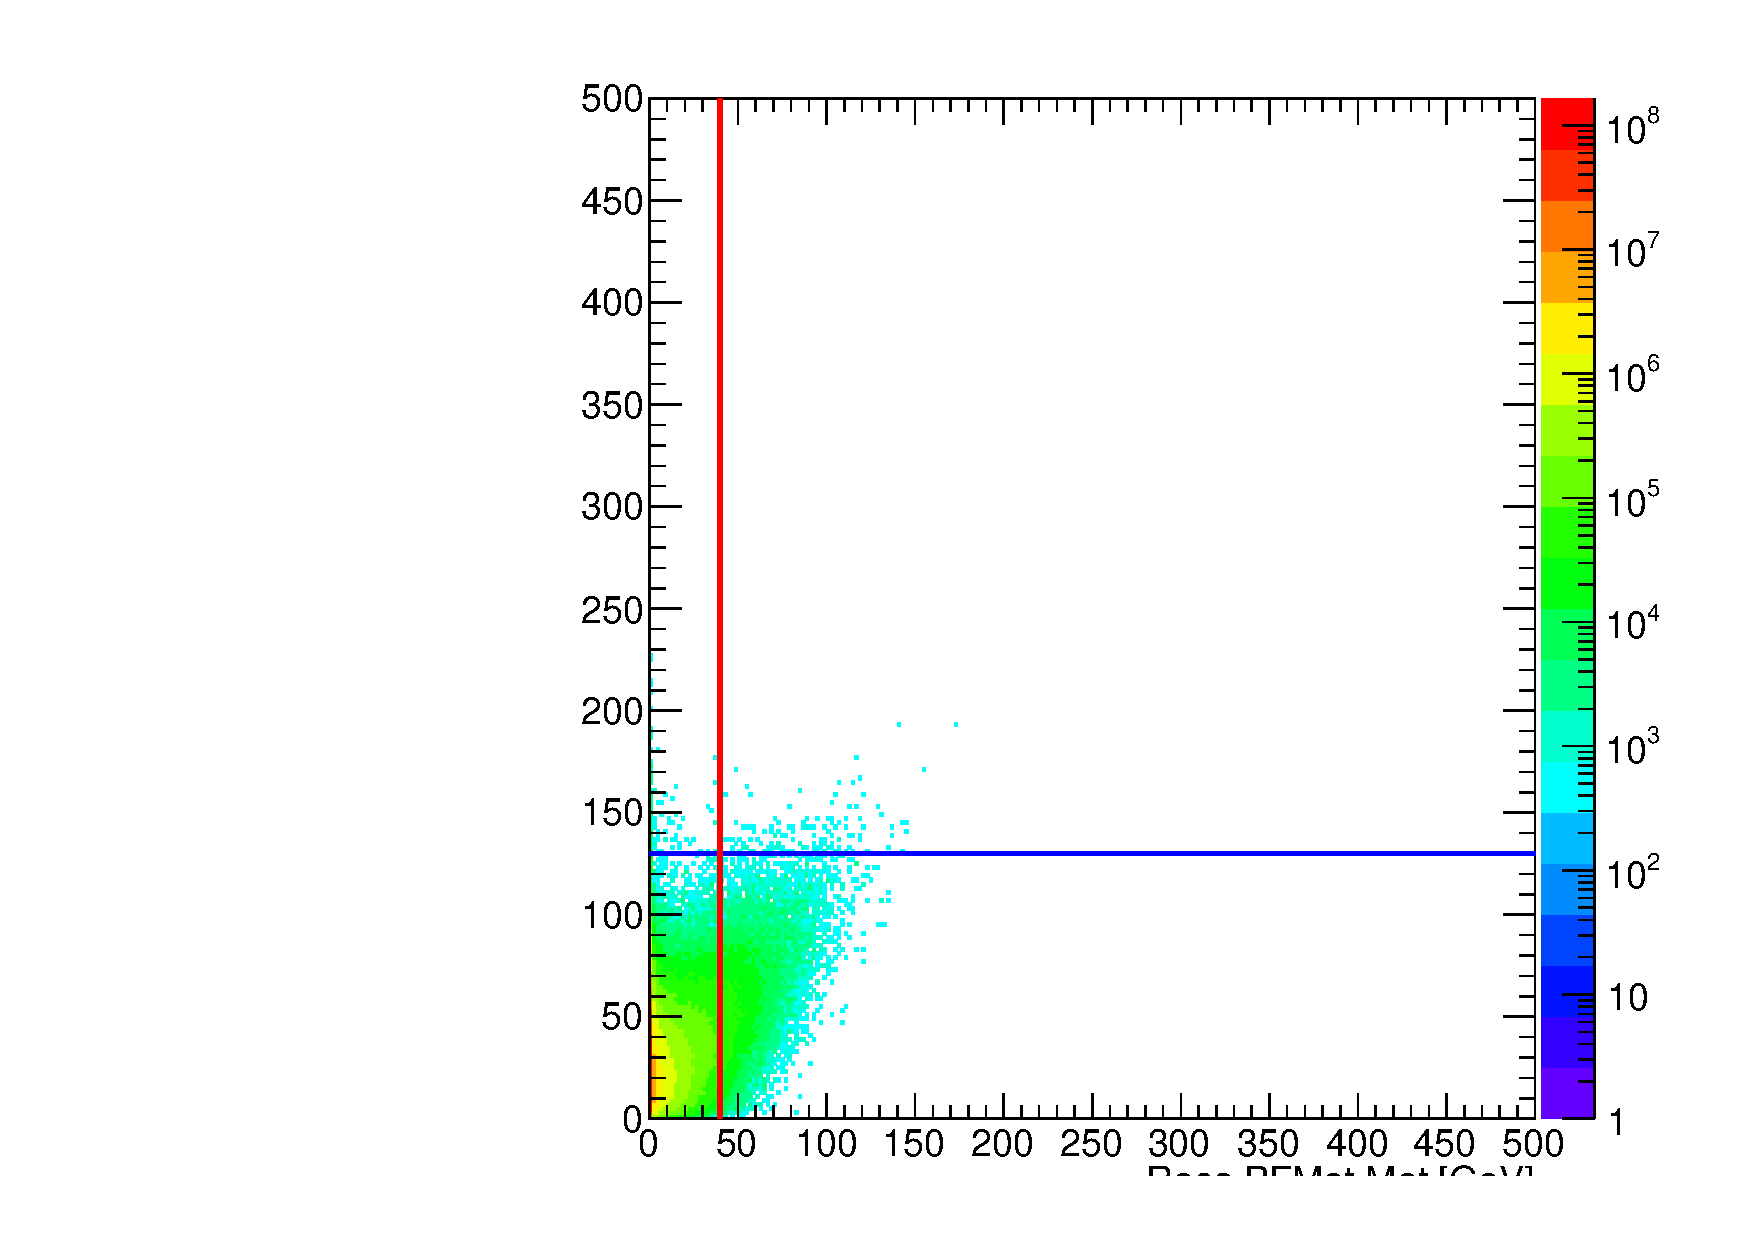
\includegraphics[width=\linewidth]{img/MC_QCD-Pt-120to170-pythia6_GenVsReco_met}

\end{block}

\end{columns}

For both this $p_T$ hats most event fall on zone C or D and are rejected analysis cut.

\end{frame}

% ###################################################
\begin{frame}{Gen Met Vs Reco MET II}

Plots here do now have any weighting but cross section since filters will operate over genEvents with no weigting this (so this is just a scaling).

\begin{columns}

\column[t]{0.45\linewidth}  
\begin{block}{170to300}
 
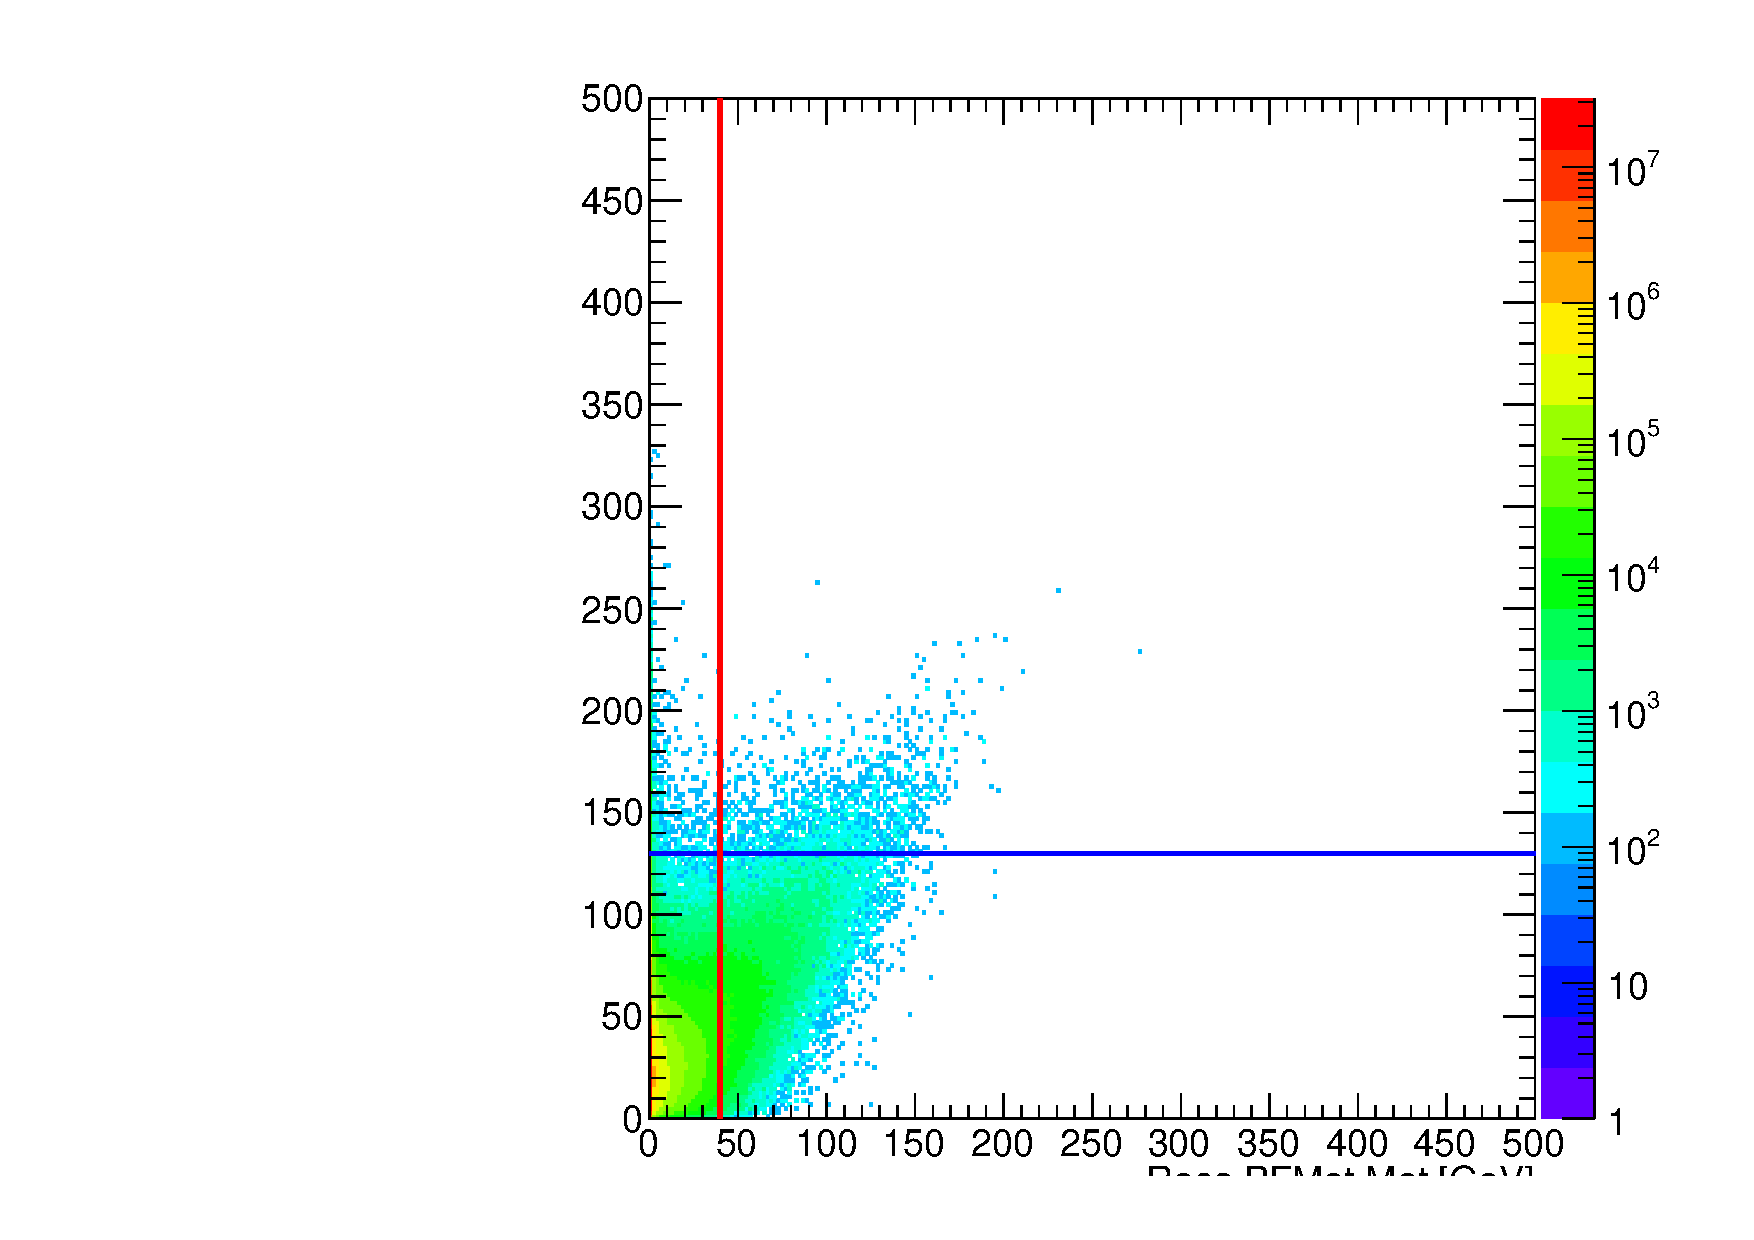
\includegraphics[width=\linewidth]{img/MC_QCD-Pt-170to300-pythia6_GenVsReco_met}
 
\end{block}


\column[t]{0.45\linewidth}  
\begin{block}{300to470}
 
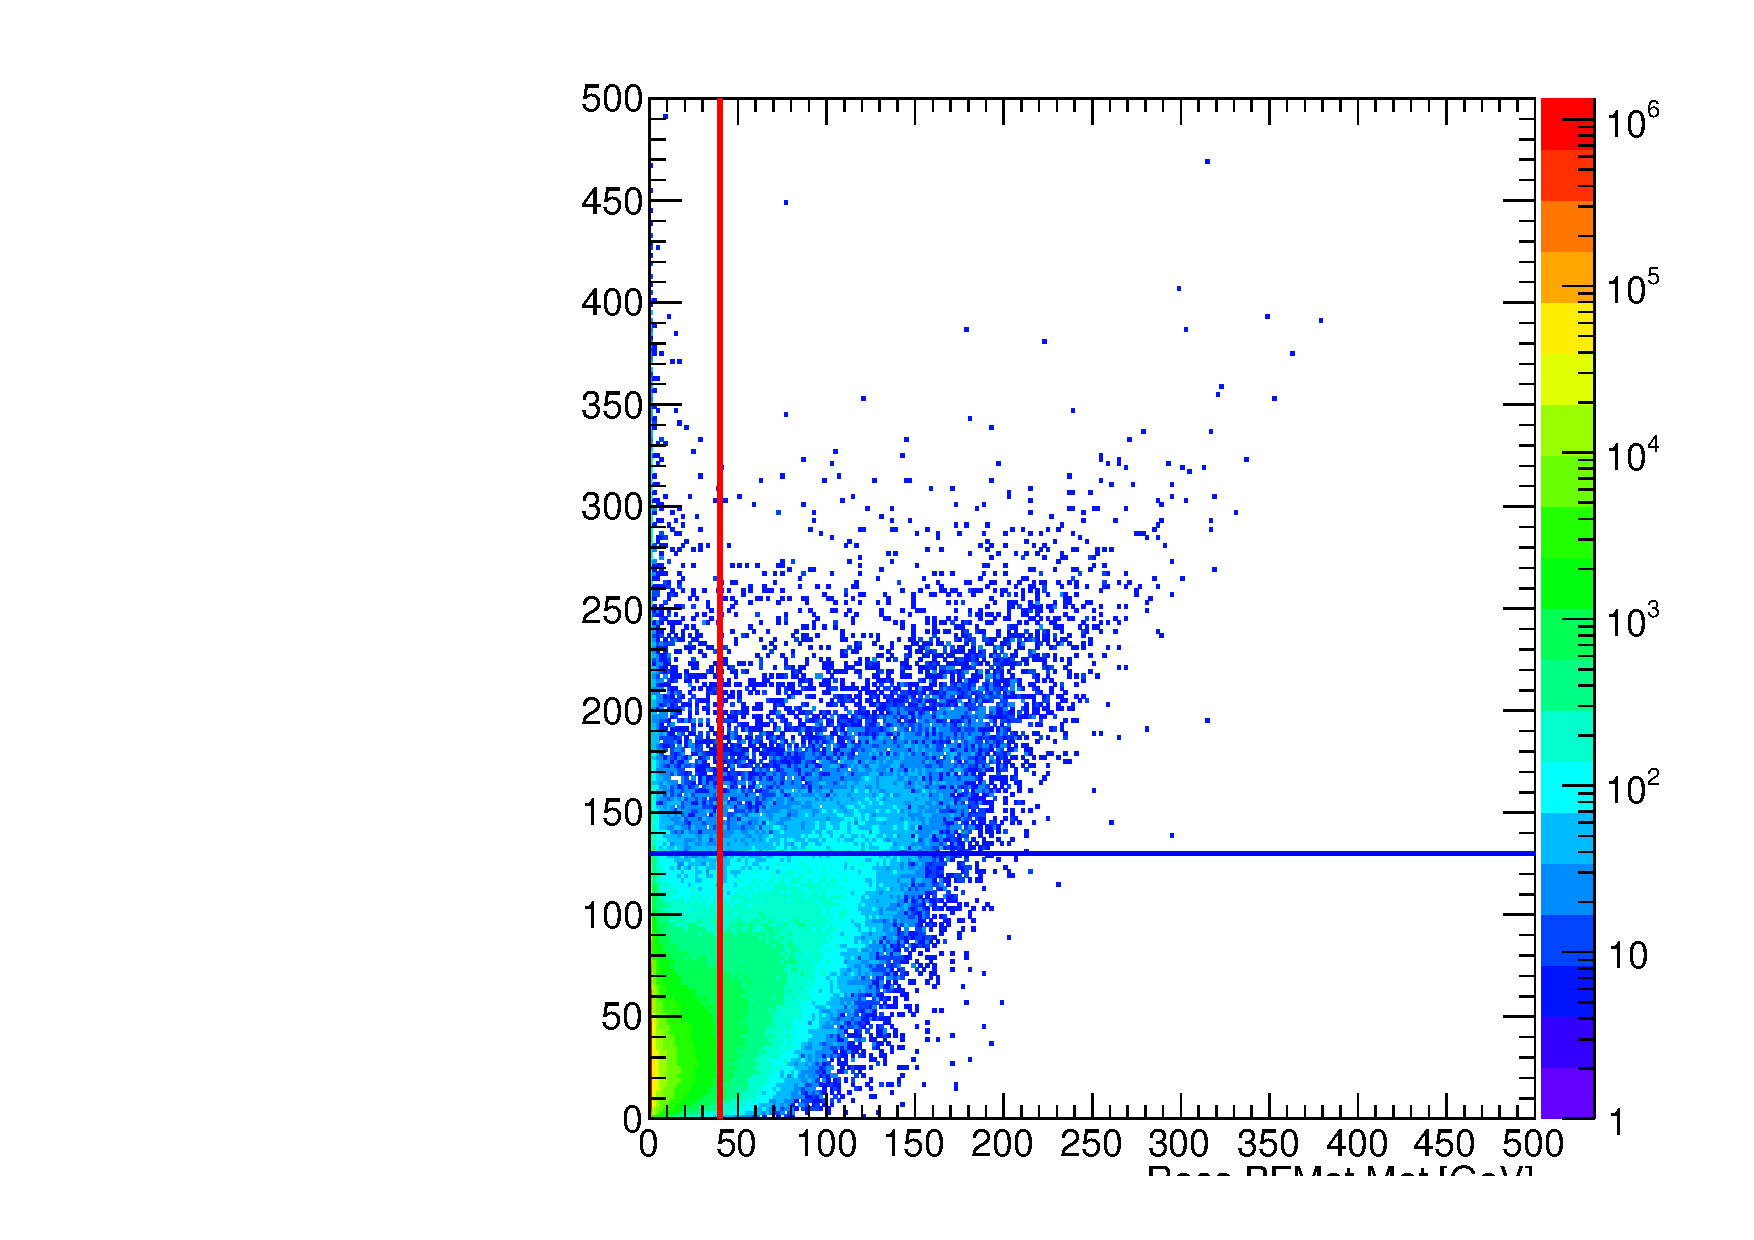
\includegraphics[width=\linewidth]{img/MC_QCD-Pt-300to470-pythia6_GenVsReco_met}

\end{block}

\end{columns}

We can se for this $p_T$ hats a significant population of events now in areas A and B.

\end{frame}

% ###################################################
\begin{frame}{Gen Met Vs Reco MET III}

Plots here do now have any weighting but cross section since filters will operate over genEvents with no weigting this (so this is just a scaling).
Plot on the right Adds all the QCD inclusive $p_T$ hats taking into account the relative cross section.

\begin{columns}

\column[t]{0.45\linewidth}  
\begin{block}{470to600}
 
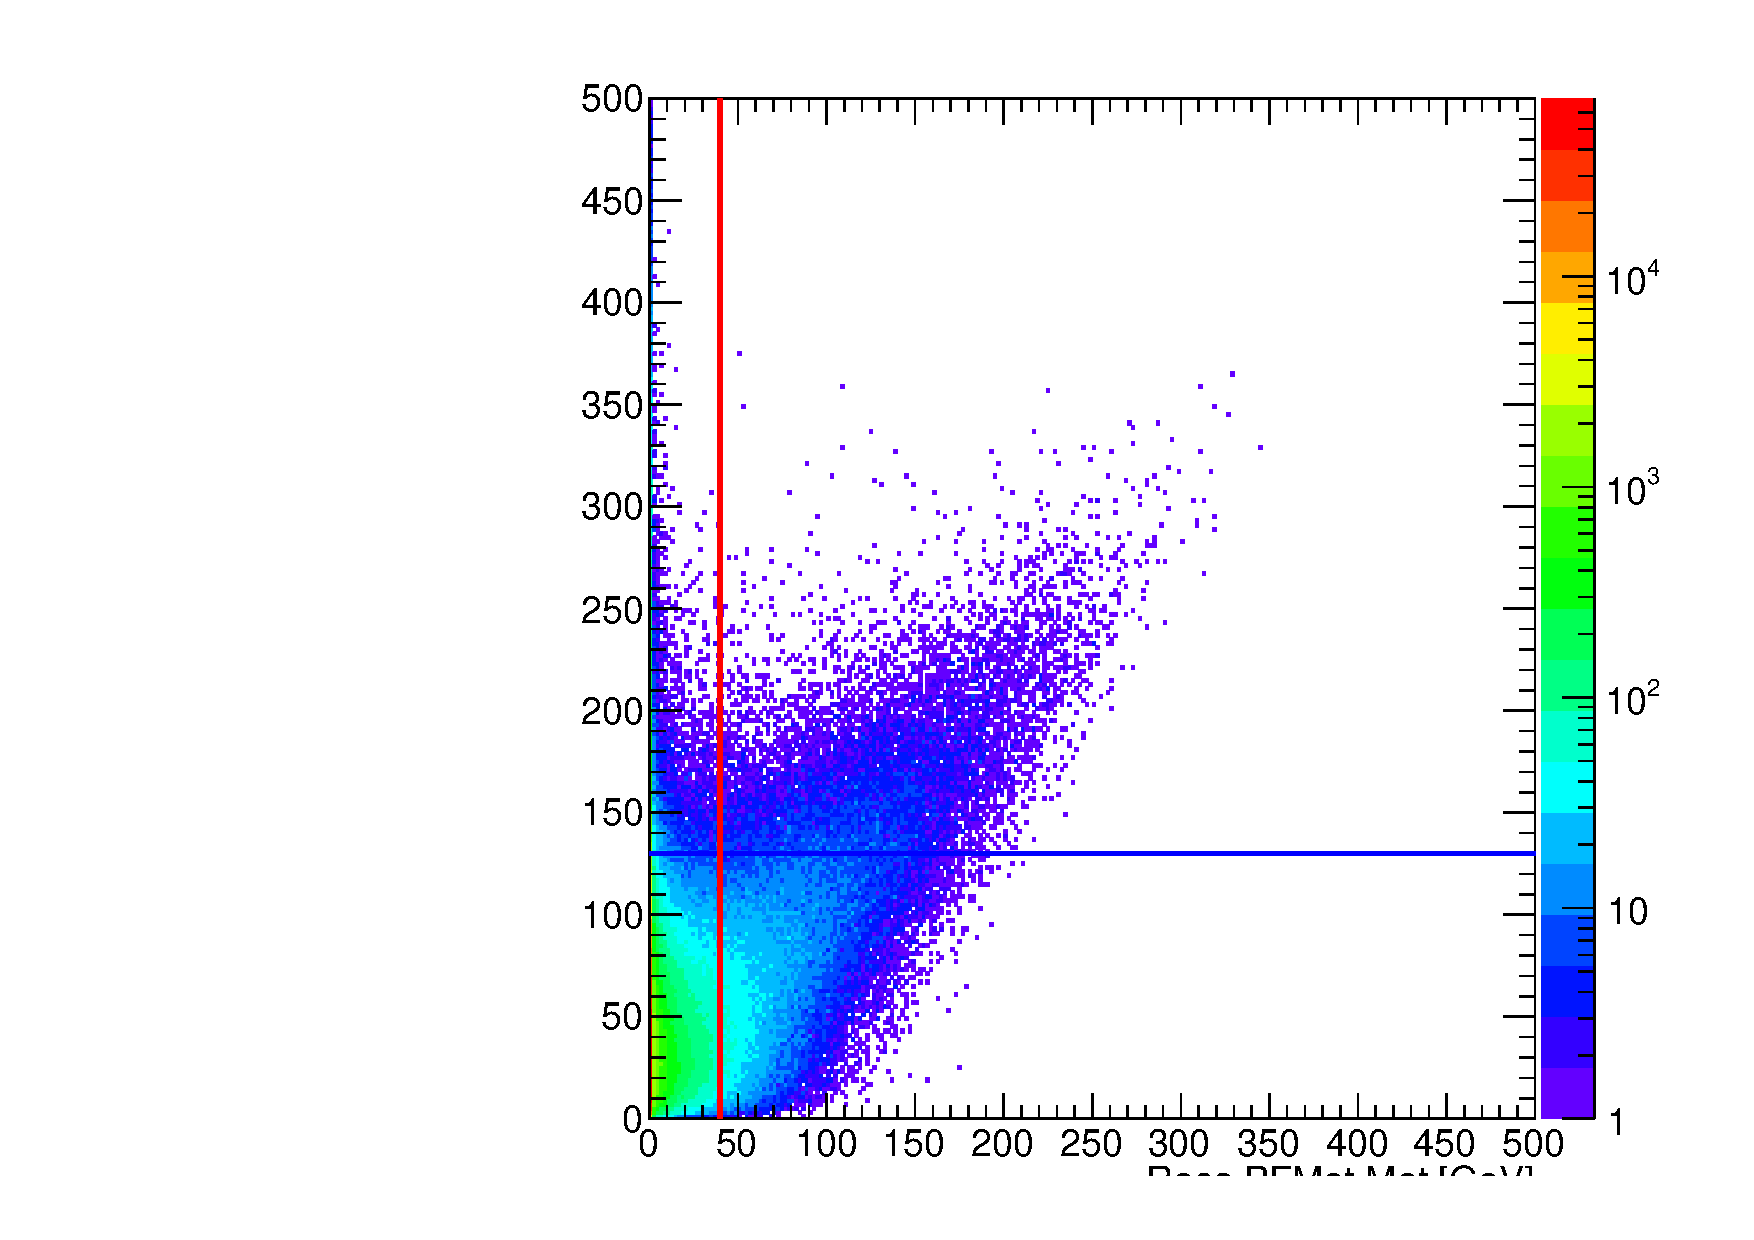
\includegraphics[width=\linewidth]{img/MC_QCD-Pt-470to600-pythia6_GenVsReco_met}

\end{block}

\column[t]{0.45\linewidth}  
\begin{block}{Total}
 
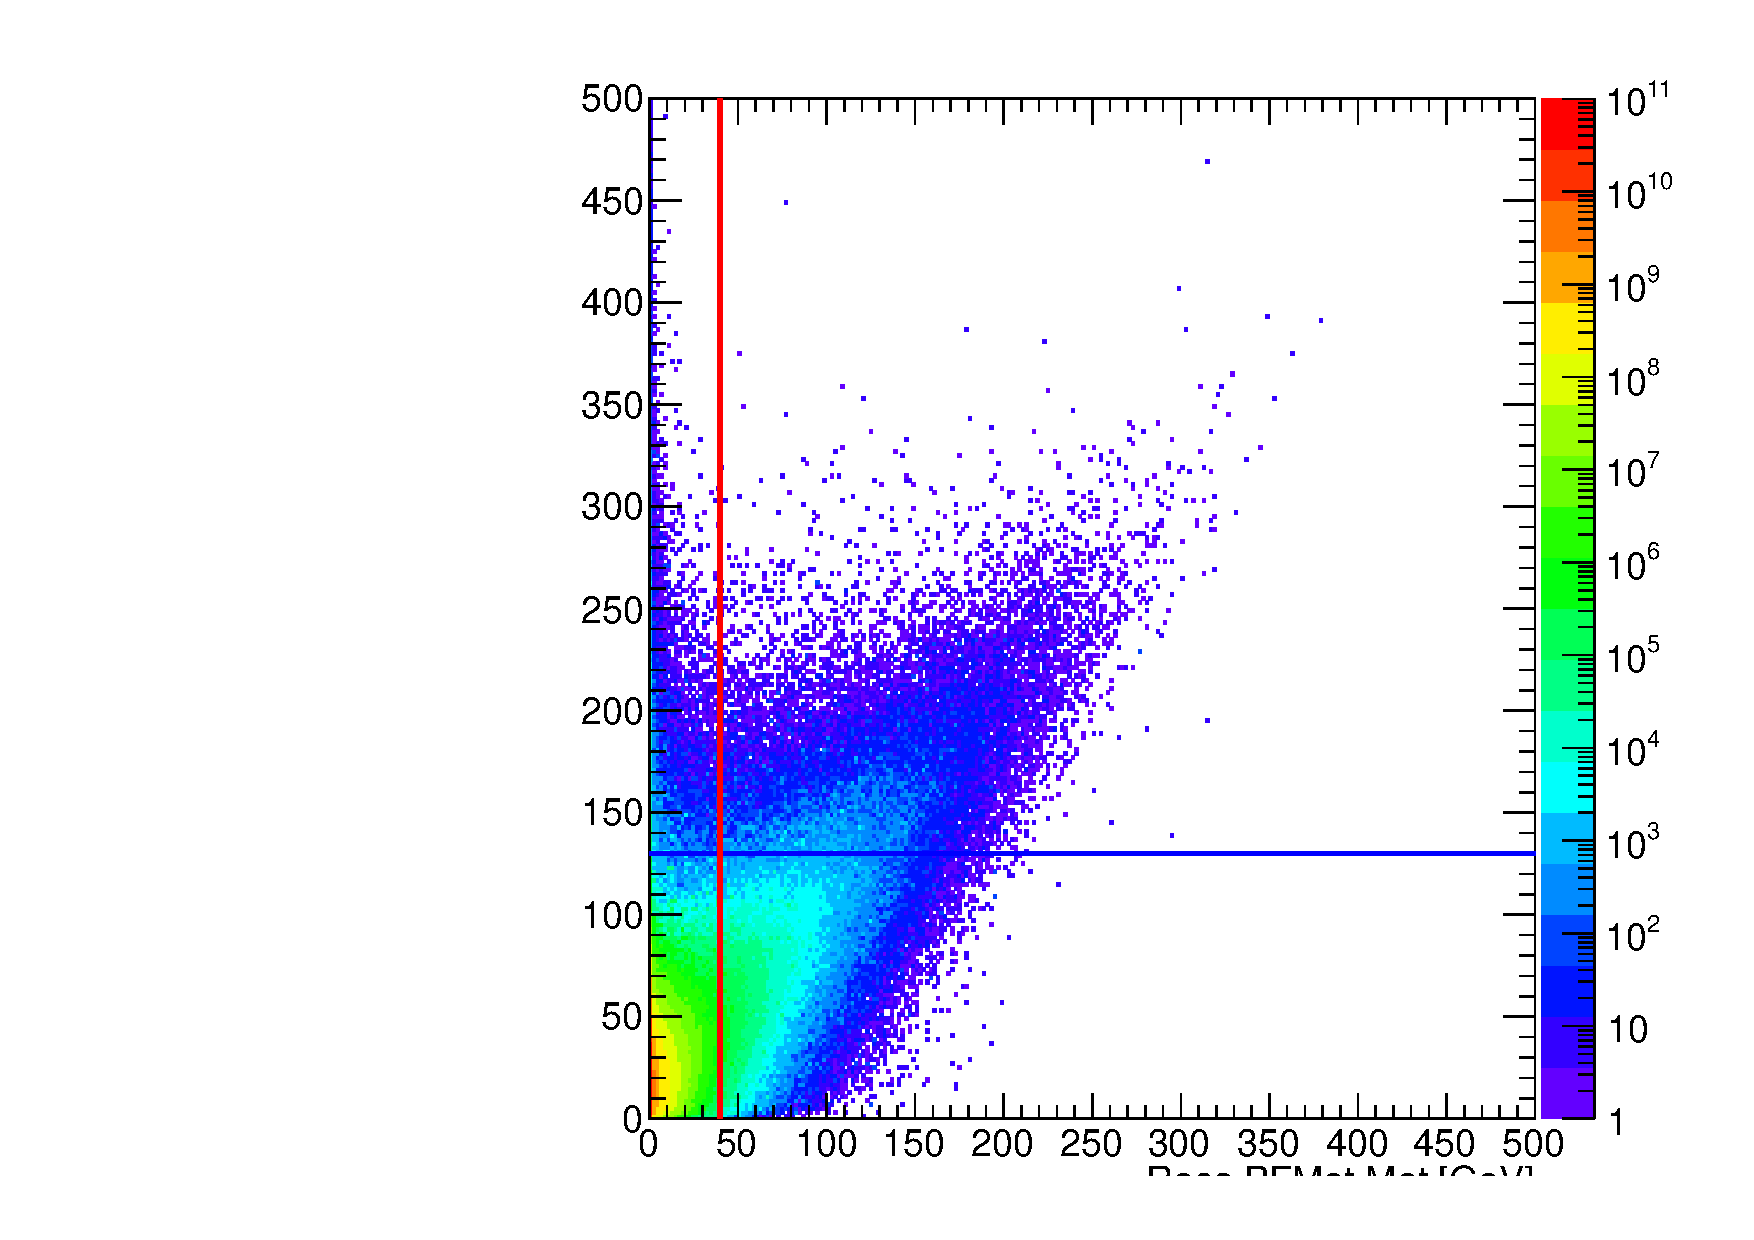
\includegraphics[width=\linewidth]{img/MC_QCDIncAll_GenVsReco_met}
 
\end{block}

\end{columns}

We can see in both plots that there is a significant population in both areas A and B.

\end{frame}

\end{document}